\documentclass[cn,10pt,math=newtx,citestyle=gb7714-2015,bibstyle=gb7714-2015]{elegantbook}

\title{家用实变函数实用技术手册}
\subtitle{Written by \LaTeX}

\author{dry}
\institute{Department of Mathematics}
\date{\today}
\version{$\mu$} 

\extrainfo{大学功夫即是明明德, 明明德只是固诚意, 诚意的工夫只是格物致知.}

\logo{shulogo.pdf}
\cover{xx3.png}

% 本文档命令
\usepackage{array}
\newcommand{\ccr}[1]{\makecell{{\color{#1}\rule{1cm}{1cm}}}}
\definecolor{customcolor}{RGB}{0,47,167} %International Klein blue
%\definecolor{customcolor}{RGB}{32,178,170}
\colorlet{coverlinecolor}{customcolor}

\usepackage{amssymb}
\usepackage{esint}
\usepackage{extarrows}
%%%%%%%%%%%%%%%%%%%%%%%%%%%%%%%%%tikz设置%%%%%%%%%%%%%%%%%%%%%%%%%%%%%%%%%%
\usepackage{tikz}
\usetikzlibrary{positioning, shapes.geometric}
\usetikzlibrary{plotmarks}
\usepackage{pgfplots}

%\usepackage{marvosym}
\usepackage{tikzsymbols}
%%%%%%%%%%%%%%%%%%%%%%%%%%%%%%%%%俄语设置%%%%%%%%%%%%%%%%%%%%%%%%%%%%%%%%%%
\usepackage{fontspec}
\newfontfamily\ru{CMU Serif}

\setmainfont{CMU Serif}
\setsansfont{CMU Sans Serif}
%%%%%%%%%%%%%%%%%%%%%%%%%%%%%%%%%水印设置%%%%%%%%%%%%%%%%%%%%%%%%%%%%%%%%%%
\usepackage{draftwatermark, everypage}
%\SetWatermarkText{瞧本环奈}
\SetWatermarkLightness{0.94}
\SetWatermarkScale{1}
%%%%%%%%%%%%%%%%%%%%%%%%%%%%%%%%%鸭子设置%%%%%%%%%%%%%%%%%%%%%%%%%%%%%%%%%%
\usetikzlibrary{ducks} 

\setcounter{tocdepth}{2} %目录深度到 subsection 层级

\begin{document}

\maketitle
\frontmatter

\chapter*{前言}
\markboth{Introduction}{前言}

随着人们生活水平的不断提高,实变函数迅速走进千家万户,越发广泛广泛应用在人们的日常生活中。

由于实变函数所涉及的内容较多,学习者不仅要懂得大定理,更要懂得大定理的用处,这对初学者来说是一个不小的挑战。
如何能快速把握实变函数学习脉络、准确掌握定理证明,这成为学习者首先要面对的问题。

出于解决以上问题,笔者在瞎编《家用实变函数实用技术手册》时参考了几种主流教材 
\cite{b1,b2,b3,b4,b5},对定理的证明与用处进行了梳理,力图做到简洁明了、举重若轻. 
应该足以应付家庭生活查阅使用,希望你能看得开心!
\Winkey[1.3][yellow]

由于时间关系, 前两章内容暂缓编写. 

\vskip 0.3cm
\underline{本书仅作个人复习查阅使用, 勿作他用!}

\vskip 0.3cm
\underline{时间仓促,文中难免有这样那样的不妥,请给予批评指正!}
数学上的错误也好,文法标点上的也好,还请不吝指教。
联系QQ:
\href{https://qm.qq.com/cgi-bin/qm/qr?k=X3d1i1X40fk58mc50cE9P6d_nBPJRDm1&noverify=0}{2155659575},
当然你也可以通过该QQ号对应的邮箱来联系笔者。


\vskip 1.5cm

\begin{flushright}
dry \\
\today 
\end{flushright}

\vskip 2.5cm
\begin{center}
	% \rule[水平高度]{长度}{粗细}
	% {\noindent} 指消除缩进
	{\noindent}\rule[-10pt]{17.5cm}{0.05em}
\end{center}
\vskip 0.5cm

Littlewood的实分析三原则是J. E. Littlewood的启发式教学法, 
用于帮助教授度量理论的要点.

\begin{table*}[htbp]
	\centering
	\begin{tabular}{l}
		\toprule
			Littlewood三原则 \\
		\midrule
			1.每个(可测)集近于区间的有限并;\\
			2.每个(可测)函数近于连续函数; \\
			3.每个收敛的(可测)函数序列近于一致收敛. \\
		\bottomrule
	\end{tabular}
\end{table*}

其中后两个原则分别来自
\ru\text{Лузин}定理(Thm:\ref{thm:Lusin1})
与\ru\text{Егоров}定理(Thm:\ref{thm:Egoroff}) , 
而可测集类可以表示为$G_{\delta}$集挖去一个零测集. 

%%%%%画 几 只 鸭 子%%%%%% 
\begin{figure}[b]

\raggedleft

\begin{tikzpicture}[scale = 1] 
	\draw (0,0) pic[ duck/water=green, duck/alien, duck/speech=Hello!, duck/laughing] {duck};
	\duck[graduate=gray!20!black, tassel=red!70!black, tshirt, jacket=gray, tie, book=\scalebox{0.25}{\tiny \TeX} , 
			xshift=60pt, scale=.3, yshift=100pt]
	\duck[tshirt=cyan, aodai=blue!50!black, conicalhat=brown, 
			xshift=90pt, scale=.3, yshift=150pt] 
	\duck[witch=black!50!gray, longhair=red!80!black, jacket=black!50!gray, magicwand, think=\scalebox{0.5}{\tiny Accio}, 
			xshift=80pt, scale=.3, yshift=50pt] 
	\duck[body=pink, unicorn=magenta!60!violet, longhair=magenta!60!violet, icecream, 
			xshift=110pt, scale=.3, yshift=100pt]
\end{tikzpicture}

\end{figure}



\tableofcontents

\mainmatter

\def\R{\mathbb{R}}
\def\Q{\mathbb{Q}}
\def\C{\mathbb{C}}
\def\N{\mathbb{N}}

\def\d{\mathrm{d}}

% !Mode:: "TeX:UTF-8"
\chapter{集合与点集}




\begin{figure}[htbp]
	\centering
	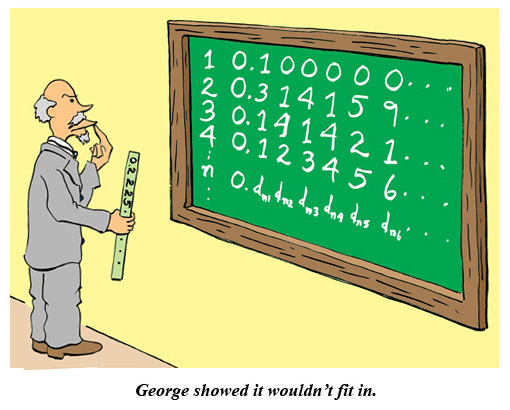
\includegraphics[scale=0.3]{figure/fitin}
\end{figure}
% !Mode:: "TeX:UTF-8"
\chapter{测度论}
% !Mode:: "TeX:UTF-8"
\chapter{可测函数}

\begin{introduction}
	\item 可测函数的定义及其性质
	\item Riesz表示定理
	\item 不同意义下的函数列收敛及其关系
	\item 可测函数与连续函数的关系
\end{introduction}
%%%%%%%%%%%%%%%%%%%%%%%%%%%%%%%%%%%%%%%%%%%%%%%%%%%%%%%%%%%%%%%%%%%%%%%%%%%%%%
%
%										下一节
%
%%%%%%%%%%%%%%%%%%%%%%%%%%%%%%%%%%%%%%%%%%%%%%%%%%%%%%%%%%%%%%%%%%%%%%%%%%%%%%

\section{可测函数的定义及其性质}


一个定义在$E \subset \R^n$上的实函数$f(x)$确定了$E$的一组子集
\begin{equation}
	E[f > a] := \{x:  x \in E , f(x) > a \},
\end{equation}
这里$a$取遍一切有限实数, 反之, $f(x)$本身也由$E$的这组子集完全确定. 
因此, 从这组子集的性质, 可以反映出$f(x)$的性质. 

\begin{definition}[可测函数]
	设$f(x)$是定义在可测集$E \subset \R^n$上的实值函数. 若对于\textbf{任意}有限实数$a$, $E[f>a]$都是可测集, 则称$f(x)$为$E$的\textbf{可测函数}.  
\end{definition}

可以证明, 对于任意有限实数$a$, 下述任一一组集合可测都是$f(x)$在$E$上可测的充要条件:
\begin{enumerate}
	\item $E[f \leq a] = E \backslash E[f>a]$; 
	\item $E[f \geq a] = \bigcap_{n=1}^{\infty} E \left[f > t-\frac 1n \right]$; 
	\item $E[f < a] = E \backslash E[f \geq a]$. 
\end{enumerate}

特别的, $f(x)$为有限函数时, $f$在$E$上可测的充要条件可以写作: 对于任意有限实数$a,b \; (a<b)$, $E[a \leq f < b]$均可测. 
\begin{proof}
	必要性显然. 
	由$b$的任意性, 任取$n \in \N^*$, 令$b = a+n$, 
	故$E[a \leq f < a+n]$可测. 
	当$f(x)$为有限函数时, 有
	$$
		E[f \geq a] = \bigcup\limits_{n = 1}^{\infty} E[a \leq f < a+n]
	$$
	可测, 因此$f$在$E$上可测. 
\end{proof}

\begin{corollary}
	设$f(x)$在$E$上可测, 则$E[f = a]$总可测, 
	任意$a \in \R \cup \{ +\infty \} \cup \{ -\infty \}$. 
\end{corollary}
\begin{proof}
	只需注意
	$$
		E[f = a] = E[f \geq a] \backslash E[f > a],
	$$
	和
	$$
		E[f = +\infty] = \bigcap\limits_{n = 1}^{\infty} E[f > n], \quad
		E[f = -\infty] = \bigcap\limits_{n = 1}^{\infty} E[f <-n].
	$$
\end{proof}

\begin{theorem}[可测函数的简单性质]
	\begin{enumerate}
		\item 设$f(x)$为$E$上的可测函数, $A$为$E$的可测子集, 则$f: A \to \R$也是可测函数;
		\item 设$E_1,E_2,\cdots,E_s$为可测集, $E = \bigcup_{i = 1}^s E_i$, 则
		$$
			f\text{为}E\text{上的可测函数} \Leftrightarrow f\text{为}E_i\text{上的可测函数}, i = 1,2,\cdots,s.
		$$
	\end{enumerate}
\end{theorem}

\begin{proof}
	\begin{enumerate}
		\item 对任意实数$a$, $A[f > a] = A \cap E[f > a]$;
		\item 对任意实数$a$, 有
		$$
			E[f > a] = \bigcup\limits_{i = 1}^s E_i[f > a].
		$$
	\end{enumerate}
\end{proof}

\begin{theorem}[可测函数的代数运算]
	设$f(x),g(x)$为$E$上广义实值可测函数, 则下列函数
	\begin{enumerate}
		\item $c f(x), \; c \in \R$; 
		\item $| f(x) |$; 
		\item $\frac{1}{f(x)}$; 
		\item $f(x) + g(x)$;
		\item $f(x) \cdot g(x)$
	\end{enumerate}
	都是$E$上的可测函数. 
\end{theorem}

\begin{theorem}[可测函数列的极限]
	设$\{ f_n(x) \}$为$E$上的一个可测函数, 则下列函数
	$$
		(\mathrm{i})   \sup\limits_{n \geq 1} f_n (x) , \;
		(\mathrm{ii})  \inf\limits_{n \geq 1} f_n (x) , \;
		(\mathrm{iii}) \varlimsup\limits_{n \to \infty} f_n (x), \;
		(\mathrm{iv})  \varliminf\limits_{n \to \infty} f_n (x). 
	$$
	都是$E$上的可测函数. 
\end{theorem}
\begin{proof}
	\begin{enumerate}
		\item[(i)]   对任意实数$a$, $E \left[\sup\limits_{n \geq 1} f_n (x) > a \right] = \bigcup\limits_{n = 1}^{\infty} E[f_n (x) > a]$; 
		\item[(ii)]  对任意实数$a$, $E \left[\inf\limits_{n \geq 1} f_n (x) < a \right] = \bigcup\limits_{n = 1}^{\infty} E[f_n (x) < a]$;
		\item[(iii),(iv)] 只须注意到$\varlimsup\limits_{n \to \infty} f_n (x) =  \sup\limits_{n \geq 1}\left(\inf\limits_{m \geq n}  (f_m (x))\right), \; \varliminf\limits_{n \to \infty} f_n (x) =  \inf\limits_{n \geq 1}\left(\sup\limits_{m \geq n}  (f_m (x))\right)$. 
	\end{enumerate}
\end{proof}
\begin{corollary}
	设$\{ f_n(x) \}$为$E$上的可测函数列, 且有
	$$
		\lim\limits_{n \to \infty} f_n(x) = f(x), \; x \in E,
	$$
	则$f(x)$为$E$上的可测函数.
\end{corollary}

\begin{definition}[几乎处处]
	设有一个与集合$E \subset \R^n$中的点$x$有关的命题$P(x)$, 
	若除了$E$中的一个零测集以外, $P(x)$皆为真,
	则称$P(x)$在$E$上\textbf{几乎处处}是真的, 
	并简记为$P(x)$ a.e.于$E$. 
\end{definition}

\begin{theorem}
	设$f(x),g(x)$是定义在$E \subset \R^n$上的广义实值函数, $f(x)$是$E$上的可测函数. 若$f(x) = g(x)$, a.e.$x \in E$,则$g(x)$在$E$上可测.
\end{theorem}
\begin{proof}
	令$A = \{ x: f(x) \neq g(x) \}$, 则$mA = 0$且$E \backslash A$是可测集. 
	对任意$a \in \R$, 我们有
	$$
	\begin{aligned}
		E[g > a] 
		& = (E \backslash A)[g>a] \cup A[g>a] \\
		& = (E \backslash A)[f>a] \cup A[g>a] .
	\end{aligned}
	$$
	由于$f$可测, $m(A[g>a]) = 0$, 从而$E[g > a]$可测. 
\end{proof}

由此可知, 对一个可测函数来说, 当改变它在零测集上的值时不会改变函数的可测性. 

\begin{definition}[简单函数]
	设$f(x)$是$E$上的实值函数. 若
	$$
		\{ y: y = f(x), x \in E \}
	$$
	为有限集, 则称$f(x)$为$E$上的\textbf{简单函数}. 
\end{definition}
设$f(x)$是$E$上的简单函数, 且有
$$
	\begin{aligned}
		& E = \bigcup\limits_{i=1}^s E_i, \; E_i \cap E_j = \varnothing, \\
		& f(x) = c_i, \; x \in E_i
	\end{aligned}
	\quad i,j = 1,2,\cdots,s
$$
此时可将$f$记作
\begin{equation}
	f(x) = \sum\limits_{i=1}^s c_i \chi_{E_i}(x), \; x \in E. \label{eq:simF}
\end{equation}
从而简单函数是有限个特征函数的线性组合. 
若$f(x)$是$E$上的简单函数, 且(\ref{eq:simF})式中的每个$E_i$都是可测集, 则称$f(x)$是$E$上的\textbf{可测简单函数}.

\begin{theorem}[Riesz表示定理] \label{thm:Riesz1}
	\begin{enumerate}
		\item[(i)] 若$f(x)$是$E$上的非负可测函数, 则存在非负可测的简单函数渐升列$\varphi_k(x) \leq \varphi_{k+1}(x),\; k=1,2,\cdots$, 使得
		$$
			\lim\limits_{k \to \infty} \varphi_k(x) = f(x),\; x \in E.
		$$
		\item[(ii)] 若$f(x)$是$E$上的可测函数, 则存在可测简单函数列$\{ \varphi_k(x) \}$满足$|\varphi_k(x) | \leq |f(x)|$, 使得
		$$
			\lim\limits_{k \to \infty} \varphi_k(x) = f(x),\; x \in E.
		$$
		若$f(x)$还是\textbf{有界}的, 则上述收敛是\text{一致}的. 
	\end{enumerate}
\end{theorem}

\begin{proof}
	\begin{enumerate}
		\item[(i)] 
		作任意的自然数$k$, 将$[0,k]$划分为$k 2^k$份, 并记
		$$
		\begin{aligned}
			& E_{k,j} = E \left[ \frac{j-1}{2^k} \leq f(x) < \frac{j}{2^k} \right], \\
			& E_k = E[f(x) \geq k], \\
			& j = 1,2,\cdots,k 2^k,\; k = 1,2,\cdots .
		\end{aligned}
		$$
		作函数列
		$$
			\varphi_k(x) = 
			\begin{cases}
				\frac{j-1}{2^k},\; x \in E_{k,j} ;\\
				k, \quad x \in E_k .
			\end{cases}
		$$
%		即
%		$$
%			\varphi_k(x) = k \chi_{E_k}(x) + \sum\limits_{j=1}^{k2^k} \frac{j-1}{2^k} \chi_{E_{k,j}}(x), \; x \in E.
%		$$
		显然, 每个$\varphi_k(x) $都是非负可测简单函数, 且满足
		$$
			\varphi_k(x) \leq \varphi_{k+1}(x) \leq f(x), \;
			\varphi_k(x) \leq k, \; k=1,2,\cdots.
		$$
		
		现在对任意的$x \in E$, 若$f(x) \neq + \infty$, 则当$k > f(x)$时有
		$$
			0 \leq f(x) - \varphi_k(x) \leq 2^{-k};
		$$
		若$f(x) = + \infty$, 则$\varphi_k(x) = k,\;(k=1,2,\cdots)$, 从而得
		$$
			\lim\limits_{k \to \infty} \varphi_k(x) = f(x), \; x \in E.
		$$
	\end{enumerate}
		
		
		\begin{enumerate}
			\item[(ii)] 
		作$f^+ (x) = \max\{f(x),0\}, f^-(x) = \min\{-f(x),0\}$, 
		从而$f(x) = f^+ (x) - f^-(x)$. 
		由(i)知, 存在非负可测简单函数列
		$\{ \varphi^{(1)}_k (x) \}$及$\{ \varphi^{(2)}_k (x) \}$满足
		$$
			\lim\limits_{k \to \infty} \varphi^{(1)}_k(x) = f^+ (x), \;
			\lim\limits_{k \to \infty} \varphi^{(2)}_k(x) = f^+ (x).
		$$
		显然$\varphi^{(1)}_k (x) - \varphi^{(2)}_k (x)$为是可测简单函数, 且有
		$$
			\lim\limits_{k \to \infty} [\varphi^{(1)}_k (x) - \varphi^{(2)}_k (x)] = f^+ (x) - f^- (x) = f(x), \; x \in E.
		$$
		若在$E$上有$| f(x) | < M$, 则当$k > M$时, 有
		$$
		\begin{aligned}
			\sup \left\{ |f^+ (x) - \varphi^{(1)}_k (x)|: x \in E \right\} < \frac{1}{2^k}, \\
			\sup \left\{ |f^- (x) - \varphi^{(2)}_k (x)|: x \in E \right\} < \frac{1}{2^k}.
		\end{aligned}
		$$
		从而知$\varphi^{(1)}_k (x) - \varphi^{(2)}_k (x)$是一致收敛于$f(x)$的.
		\end{enumerate}
		
\end{proof}


%%%%%%%%%%%%%%%%%%%%%%%%%%%%%%%%%%%%%%%%%%%%%%%%%%%%%%%%%%%%%%%%%%%%%%%%%%%%%%
%
%										下一节
%
%%%%%%%%%%%%%%%%%%%%%%%%%%%%%%%%%%%%%%%%%%%%%%%%%%%%%%%%%%%%%%%%%%%%%%%%%%%%%%

\section{不同意义收敛的可测函数列}

%%%%%%%%%%%%%%%%%%%%%%%%%%%%%%%%%%%%%%%%%%%%%%%%%%%%%%%%%%%%%%%%%%%%%%%%%%%%%%
\subsection{不同意义下的收敛}

给定一个函数列, 在考虑它的收敛问题时, 我们一般考虑以下几种收敛: 
\begin{definition}[一致收敛]
	$\{ f_n(x) \}$为定义在$E \subset \R^n$上的函数列, 若对任意的$\varepsilon > 0$, 恒有只依赖于$\varepsilon$的正整数$N(\varepsilon)$, 使得$n > N(\varepsilon)$时, 若有
		\begin{equation}
			\left| f_n(x) - f(x) \right| < \varepsilon, \forall x \in E.
		\end{equation}
		恒成立, 则称$f_n(x)$在$E$上一致收敛于$f(x)$. 
\end{definition}

\begin{definition}[近一致收敛]
	称$f_n(x)$在$E$上近一致收敛于$f(x)$, 如果任给$\delta > 0$, 存在$E$的可测子集$E_{\delta}$使得$\{ f_n(x) \}$在$E_{\delta}$上一致收敛于$f(x)$, 而$m (E \backslash E_{\delta} ) < \delta$. 
\end{definition}

\begin{definition}[a.e.收敛]
	称$f_n(x)$在$E$上a.e.收敛于$f(x)$, 如果任给$\varepsilon > 0$, 有
	\begin{equation}
		m E\left[ \lim\limits_n |f_n - f| \geq \varepsilon \right] = 0.
	\end{equation}
\end{definition}

\begin{definition}[依测度收敛]
	称$f_n(x)$在$E$上依测度收敛于$f(x)$, 如果任给$\varepsilon > 0$, 有
	\begin{equation}
		\lim\limits_n m E\left[ |f_n - f| \geq \varepsilon \right] = 0.
	\end{equation}
\end{definition}

依测度收敛是一种什么样的收敛呢? 
用文字来叙述, 
就是说如果事先给了一个(误差)$\varepsilon>0$, 不管这个 $\varepsilon$ 有多小, 
使得$\left|f_{n}(x)-f(x)\right|$大于(误差)$\varepsilon$的点$x$虽然可能很多, 
但这种点$x$的全体的测度却是随着 $n$ 无限地增大而趋向于零.

在概率论中, 常用$\mu$表示概率, 这时依测度收敛改称为依概率收敛. 

下面我们先举两个反例, 来说明这种收敛概念和我们所熟悉的处处收敛或 a.e.收敛概念是有很大区别的.
%%%%%%%%%%%%%%%%%%%%%%%%%%%%%%%%%%%%%%%%%%%%%%%%%%%%%%%%%%%%%%%%%%%%%%%%%%%%%%
\subsection{两个反例}

\begin{example}
	\framebox[\width]{依测度收敛而处处不收敛的函数列} \par 
	取$E = (0,1]$, 将$E$等分, 定义两个函数: 
	$$
	\begin{array}{c c}
		f_1^{(1)} = 
		\begin{cases}
			1, & x \in \left(0, \frac{1}{2} \right], \\
			0, & x \in \left(\frac{1}{2}, 1 \right],
		\end{cases}
		& 
		f_2^{(1)} = 
		\begin{cases}
			0, & x \in \left(0, \frac{1}{2} \right], \\
			1, & x \in \left(\frac{1}{2}, 1 \right].
		\end{cases}
	\end{array}
	$$
	然后将$(0,1]$四等分、八等分、……. 一般地, 对每个$n$, 作$2^n$个函数: 
	$$
	f_j^{(n)} = 
		\begin{cases}
			0, & x \in \left(\frac{j-1}{2^n}, \frac{j}{2^n} \right], \\
			1, & x \notin \left(\frac{j-1}{2^n}, \frac{j}{2^n} \right].
		\end{cases}
	\quad j = 1,2,\cdots,2^n.
	$$
	我们把$\{ f_j^{(n)},\; j = 1,2,\cdots,2^n \}$按照先$n$后$j$的顺序逐个的排成一列:
	$$
		f_1^{(1)}, f_2^{(1)}, 
		f_1^{(2)}, f_2^{(2)}, f_3^{(2)}, f_4^{(2)}, 
		\cdots, 
		f_1^{(n)}, f_2^{(n)}, \cdots, f_{2^n}^{(n)}, 
		\cdots
	$$
	其中$f_j^{(n)}$在这个序列中是第$N = 2^n - 2 +j$个函数. 
	
	我们说, 这个序列是依测度收敛于$0$的. 
	这是因为对任意的$\sigma > 0$, $E[|f_j^{(n)} - 0| \geq \sigma]$
	或是空集($\sigma >1$), 
	或是$(\frac{j-1}{2^n}, \frac{j}{2^n}] \; (0 < \sigma \leq 1)$, 
	因此
	$$
		m( E[|f_j^{(n)} - 0| \geq \sigma] ) \leq \frac{1}{2^n}. 
	$$
	由于当$N$趋于$\infty$时有$n \to \infty$, 由此可见
	$$
		\lim\limits_{N \to \infty} m( E[|f_j^{(n)} - 0| \geq \sigma] ) = 0, 
	$$
	即$f_j^{(n)}$依测度收敛于$0$. 
	但是该函数列在$(0,1]$上任何一点都不收敛! 
	事实上, 对任意$x_0 \in (0,1]$, 无论$n$多大, 总存在$j$使得
	$$
		x_0 \in \left(\frac{j-1}{2^n}, \frac{j}{2^n} \right].
	$$
	
	换言之, 对于任何的$x_0 \in (0,1]$, 
	在$\{ f_j^{(n)}(x_0) \}$中必有两子列, 一个恒为$1$, 一个恒为$0$. 
	所以该函数列在$(0,1]$上任何点都发散. 
\end{example}

反之, 一个 a.e.收敛的函数列也可以是不依测度收敛的. 

\begin{example}
	\framebox[\width]{ a.e.收敛而不依测度收敛的函数列} \par
	取$E = (0, \infty)$, 作函数列
	$$
		f_n(x) = 
		\begin{cases}
			1, & x \in (0, n], \\
			0, & x \in (n, \infty),
		\end{cases}
		\quad n = 1,2,\cdots.
	$$
	显然$f_n(x) \to 1 \; (n \to \infty)$, 
	而当$0 < \sigma < 1$时, 
	$$
		m( E[|f_n - 1| \geq \sigma] ) = m(n, \infty) = \infty.
	$$
	故$\{ f_n \}$不依测度收敛于$1$. 
\end{example}

尽管两种收敛有较大区别, 但还是有着密切联系的. 
下面我们对于各种函数列不同意义的收敛间的关系予以说明. 
%%%%%%%%%%%%%%%%%%%%%%%%%%%%%%%%%%%%%%%%%%%%%%%%%%%%%%%%%%%%%%%%%%%%%%%%%%%%%%
\subsection{不同意义收敛的关系}

\begin{center}
\begin{figure}[h!]
\begin{tikzpicture}

	\tikzstyle{every node}=[font=\small,scale=2] %放大

	\node[draw, rounded corners]                        (ccon)   {一致收敛};
	\node[draw, rounded corners, right = 90pt of ccon]  (accon)  {近一致收敛};
	\node[draw, rounded corners, above = 60pt of accon] (aecon)  {a.e.收敛};
	\node[draw, rounded corners, right = 90pt of accon] (conbm)  {依测度收敛};
	
	\tikzstyle{arrow1} = [thick,->,>=stealth]
	\draw[arrow1] (ccon)       --    (accon);
	\draw[arrow1] (ccon)       --    (aecon);
	\draw[arrow1] (206pt,16pt) --    (206pt,76pt);
	\draw[arrow1] (accon)      --    (conbm);
	
	\tikzstyle{arrow2} = [thick,cyan,->,>=stealth]
	\draw[arrow2] (163pt,76pt) --    node[left]{\tiny \ru\text{Егоров}}(163pt,16pt);
	\draw[arrow2] (aecon)      --    node[left]{\tiny Lebesgue}(conbm);
	
	\tikzstyle{arrow3} = [thick,dashed,->,>=stealth]
	\draw[arrow3] (370pt,17pt) --    node[right]{\tiny Riesz}(227pt,90pt);

\end{tikzpicture}	
\caption{不同意义收敛的可测函数列间的关系.}
\end{figure}
\end{center}

%%%%%%%%%%%%%%%%%%%%%%%%%%%%%%%%%%%%%%%%%%%%%%%%%%%%%%%%%%%%%%%%%%%%%%%%%%%%%%
\vskip 5cm
\subsection{定理及其证明}

上述中需要证明的有\ru\text{Егоров}定理及其逆定理, Lebesgue定理, Riesz定理以及近一致收敛一定依测度收敛, 其余显然. 
特别的, 我们此处对于Lebesgue定理的证明由\ru\text{Егоров}定理与近一致收敛一定依测度收敛两部分组成, 因此不再对近一致收敛一定依测度收敛另作证明.

\vskip 0.2cm
\begin{theorem}[\ru\text{Егоров}定理]\label{thm:Egoroff}
	设$mE < \infty$, $\{ f_n \}$是$E$上一列$a.e.$收敛于一个$a.e.$有限的函数$f$的可测函数, 那么对于任意$\delta > 0$, 存在子集$E_{\delta} \subset E$, 使$\{f_n\}$在$E_{\delta}$上一致收敛, 且$m(E \backslash E_{\delta}) < \delta$.
\end{theorem}

\begin{proof}
		\framebox[\width]{挖去出现无穷减无穷型未定式的零测集}

		由条件, $m\left( E[ |f_n| = \infty ] \right) = 0,\; n=1,2,\cdots$, $m( E[ |f| = \infty ] ) = 0$. 则有$mE_0 = 0$, 其中
		$$
			E_0 = \bigcup\limits_{i=1}^n E\left[ |f_n| = \infty \right] \cup E[ |f| = \infty ]\;.
		$$
	用$E \backslash E_0$代替$E$, 从而有
		$$
		\lim\limits_{n \to \infty} (f_n(x) - f(x)) = 0,\; a.e. \; x \in E.
		$$

	\framebox[\width]{构造一致收敛点集$E_k$}

	$E$上$\{ f_n \}$不收敛于$f$的点集
		$$
		E\left[ \lim\limits_{n \to \infty} (f_n - f) \neq 0 \text{或极限不存在} \right] = 
		\bigcup\limits_{k = 1}^{\infty} \bigcap\limits_{N = 1}^{\infty} \bigcup\limits_{n = N}^{\infty} E \left[ |f_n - f| \geq \frac 1k \right]
		$$
	为零测集, 那么对于任意$k$, 有
		$$
			m \left( \bigcap\limits_{N = 1}^{\infty} \bigcup\limits_{n = N}^{\infty} E \left[ |f_n - f| \geq \frac 1k \right]  \right) = 0. 
		$$
	又$mE < \infty$, 则
		$$
			\lim\limits_{N \to \infty} m \left( \bigcup\limits_{n = N}^{\infty} E \left[ |f_n - f| \geq \frac 1k \right] \right) = m \left( \bigcap\limits_{N = 1}^{\infty} \bigcup\limits_{n = N}^{\infty} E \left[ |f_n - f| \geq \frac 1k \right]  \right) = 0
		$$
	于是对于任意$\delta > 0, k \in \mathbb{N}^*$, 存在$N_k$使得$m\left( \bigcup\limits_{n = N_k}^{\infty} E \left[ |f_n - f| \geq \frac 1k \right] \right) < \frac{\delta}{2^k}$. 

	\framebox[\width]{构造$E_{\delta}$并证明$E$与其的差集的测度满足要求}

	令
		$$
			E_{\delta} = \bigcap\limits_{k = 1}^{\infty} \bigcap\limits_{n = N_k}^{\infty} E \left[ |f_n - f| < \frac 1k \right]\;.
		$$
	那么有
		$$
			\begin{aligned}
				m(E \backslash E_{\delta})
				&= m \left( \bigcup\limits_{k = 1}^{\infty} \bigcup\limits_{n = N_k}^{\infty} E \left[ |f_n - f| \geq \frac 1k \right] \right) \\
				&\leq \sum\limits_{k = 1}^{\infty} m \left(\bigcup\limits_{n = N_k}^{\infty} E \left[ |f_n - f| \geq \frac 1k \right] \right) \\
				&< \sum\limits_{k = 1}^{\infty} \frac{\delta}{2^k} = \delta\;.
			\end{aligned}
		$$

	\framebox[\width]{证明$f_n$在$E_{\delta}$上的一致收敛性}

	任取$\varepsilon > 0$, 存在$k$, 使$\frac 1k < \varepsilon$, 令$N = N_k$. 由于
		$$
			E_{\delta} \subset \bigcap\limits_{n = N_k}^{\infty} E \left[ |f_n - f| < \frac 1k \right]
		$$
	因此对于任意$n \geq N,\; x\in E_{\delta}$ , 有
		$$
			|f_n(x) - f(x) | < \frac 1k < \varepsilon
		$$
	成立, 故$\{ f_n(x) \}$在$E_{\delta}$上一致收敛于$f(x)$. 
\end{proof} 
 
\vskip 0.2cm
\begin{theorem}[\ru\text{Егоров}定理的逆定理]
	设可测函数列$\{ f_n \}$在$E$上近一致收敛于函数$f$, 则$\{ f_n \}$在$E$上a.e.收敛于函数$f$. 
\end{theorem}

\begin{proof}
	即对任意$\delta > 0$, 存在$E$的可测子集$E_{\delta}$满足$m (E \backslash E_{\delta} ) < \delta$, 使得$\{ f_n(x) \}$在$E_{\delta}$上一致收敛于$f(x)$. 

	设$E_0$为$\{ f_n(x) \}$不收敛于$f(x)$的点集, 从而$E_0 \subset E \backslash E_{\delta}$, 所以$m E_0 \leq m(E \backslash E_{\delta}) < \delta$.故$m E \to 0\; (\delta \to 0)$, 从而$\{ f_n \}$a.e.收敛于函数$f$. 
\end{proof}

\vskip 0.2cm
当然, 此处称“\ru\text{Егоров}定理的逆定理”显然是不严谨的, 
因为条件中去掉了$m E < \infty$的限制, 
但是为了方便记忆, 笔者在此给这个定理冠上了个如此的名号.

\vskip 0.2cm
\begin{theorem}[Lebesgue定理]
	设$m E < \infty$, $E$上a.e.有限的可测函数列$\{ f_n(x) \}$a.e.收敛于$f(x)$, 则$\{ f_n (x) \}$依测度收敛于$f(x)$.
\end{theorem}

\begin{proof}
	由\ru\text{Егоров}定理, 任给$\varepsilon, \delta > 0$, 存在可测集$E_{\delta} \subset E$满足$m(E \backslash E_{\delta}) < \delta$, 且存在$N$, 当$n > N$时, 有
		$$
			|f_n(x) - f(x)| < \varepsilon,\; \forall x \in E_{\delta},
		$$
	从而$E \left[ |f_n - f| \geq \varepsilon \right] \subset E \backslash E_{\delta}$, 从而有
		$$
			\lim\limits_n m(E \left[ |f_n - f| \geq \varepsilon \right]) \leq m(E \backslash E_{\delta}) < \delta.
		$$
	令$\delta \to 0$, 有$\lim\limits_n m(E \left[ |f_n - f| \geq \varepsilon \right]) = 0$, 故而$\{ f_n (x) \}$依测度收敛于$f(x)$.
\end{proof}

\begin{note}
	注意\ru\text{Егоров}逆定理与Lebesgue定理选取的不收敛点集的区别:
	\begin{enumerate}
		\item \ru\text{Егоров}逆定理
			\begin{center}
				$E_0 = E\left[ \lim\limits_n |f_n - f| \geq \varepsilon \right] \subset E \backslash E_{\delta},$ \\
				$\Rightarrow m E_0 <\delta$
			\end{center}
		\item Lebesgue定理
			\begin{center}
				$E_n = E\left[ |f_n - f| \geq \varepsilon \right] \subset E \backslash E_{\delta},$ \\
				$\Rightarrow \lim\limits_n m E_n < \delta.$
			\end{center}
	\end{enumerate}
\end{note}

\begin{theorem}[Riesz定理] \label{thm:Riesz2}
	$E$上可测函数列$\{ f_n \}$依测度收敛于$f$, 则存在子列$\{f_{n_i}\}$在$E$上a.e.收敛于$f$.
\end{theorem}

\begin{proof}
	\framebox[\width]{根据依测度收敛构造逐点不收敛集$E_s$}\par 
	对任意$s \in \mathbb{N}^*$, 取$\varepsilon = \sigma = \frac 1{2^s}$. 由$f_n(x) \Rightarrow f(x)$, 所以存在$n_s$使得
		$$
			m E_s < \frac 1 {2^s},
		$$
	其中$E_s = E \left[ | f_{n_s} - f | \geq \frac 1 {2^s} \right]$. 不妨设$n_1 < n_2 < \cdots$. 

	\framebox[\width]{构造子列收敛点集下极限$F$}\par
	令
		$$
			F_k = E \backslash \left( \bigcup\limits_{s = k}^{\infty} E_s \right) =  \bigcap\limits_{s = k}^{\infty} (E \backslash E_s) \\
			= \bigcap\limits_{s = k}^{\infty} E \left[ | f_{n_s} - f | < \frac 1 {2^s} \right].
		$$
	显然在$F_k$上, $f_{n_s} \to f$. 作$F = \bigcup\limits_{k = 1}^{\infty} F_k$, 则在$F$上有$f_{n_s} \to f$. 

	\framebox[\width]{证明$E \backslash F$测度为零}\par 
		$$
		\begin{aligned}
			E \backslash F
			&= E \backslash \bigcup\limits_{k = 1}^{\infty} \bigcap\limits_{s = k}^{\infty} E \left[ | f_{n_s} - f | < \frac 1 {2^s} \right] \\
			&= \bigcap\limits_{k = 1}^{\infty} \bigcup\limits_{s = k}^{\infty} E_s .
		\end{aligned}
		$$
	从而对任意$k$,有$E \backslash F \subset \bigcup\limits_{s = k}^{\infty} E_s$. 
	又$\sum\limits_{s = 1}^{\infty} m E_s = 1$, 那么根据Cauchy收敛准则有
		$$
		m(E \backslash F) \leq m \left(\bigcup\limits_{s = k}^{\infty} E_s \right) \leq \sum\limits_{s = k}^{\infty} m E_s \to 0 \qquad (k \to \infty).
		$$
\end{proof}

Riesz定理剔除了那些收敛速度不够快的函数项.

\vskip 0.2cm
Lebesgue定理与Riesz定理提供了处理极限与测度换序的有力工具. 

\begin{center}
\begin{figure}[h!]
\begin{tikzpicture}

	\tikzstyle{every node}=[font=\tiny,scale=2] %放大

	\node[draw, rounded corners]                        (aecon)  {a.e.收敛 \\ $\lim\limits_{n \to \infty} m E[|f_n - f| \geq \sigma]$};
	\node[draw, rounded corners, right = 60pt of aecon] (conbm)  {依测度收敛 \\ $m E[ \lim\limits_{n \to \infty} |f_n - f| \geq \sigma]$ };
	
	\tikzstyle{arrow} = [thick,->,>=stealth]
	\draw[arrow] (aecon)    --    node[above]{\tiny Lebesgue}(conbm);
	\draw[arrow] (conbm)    --    node[below]{\tiny Riesz}(aecon);


\end{tikzpicture}	
\caption{Lebesgue定理与Riesz定理在极限与测度换序中的应用.}
\end{figure}
\end{center}


%%%%%%%%%%%%%%%%%%%%%%%%%%%%%%%%%%%%%%%%%%%%%%%%%%%%%%%%%%%%%%%%%%%%%%%%%%%%%%
%
%										下一节
%
%%%%%%%%%%%%%%%%%%%%%%%%%%%%%%%%%%%%%%%%%%%%%%%%%%%%%%%%%%%%%%%%%%%%%%%%%%%%%%

\section{可测函数与连续函数的关系}

\begin{definition}[连续函数]
	称定义在$E \subset \R^n$上的实函数$f(x)$在$x_0 \in E$连续, 
	如果$y_0 = f(x_0)$有限, 
	而且对于$y_0$的任一邻域$V$, 存在$x_0$的某邻域$U$, 
	使得$f(U \cap E) \subset V$. 
	如果$f(x)$在$E$的每一点连续, 则称$f(x)$在$E$上连续.
\end{definition}

\begin{example}
	区间$[0,1]$上的Dirichlet函数
	$$
	D(x) = 
	\begin{cases}
		1, & x \in [0,1] \cap \Q, \\
		0, & x \in [0,1] \backslash \Q,
	\end{cases}
	$$
	它在$[0,1]$上没有连续点, 但是将$D(x)$限制在集合$[0,1] \backslash \Q$时, 
	所得函数为$D(x)|_{[0,1] \backslash \Q}$便是该集合上的常值函数$0$, 因而它是连续函数. 
	然而函数$D(x)|_{[0,1] \backslash \Q}$与$D(x)$定义域不同, 不是同一函数. 
\end{example}

显然,一个函数在其定义域的每一个孤立点都是连续的.
\begin{theorem}[连续函数可测]
	可测集$E \subset \R^n$上连续函数可测. 
\end{theorem}
\begin{proof}
	设$x \in E[f>a]$, 由连续性, 存在$x$的某邻域$U(x)$, 使得
	$$
		U(x) \cap E \subset E[f>a].
	$$
	因此, 令$G = \bigcup\limits_{x \in E[f>a]} U(x)$, 则
	$$
		G \cap E = \bigcup\limits_{x \in E[f>a]} U(x) \cap E \subset E[f>a].
	$$
	反之, 显然有$G \supset E[f>a]$, 因此
	$$
		E[f>a] \subset G \cap E[f>a] \subset G \cap E,
	$$
	从而$E[f>a] = G \cap E$. 但$G$为开集, 故$G \cap E$仍然可测. 
\end{proof}

反之, 一般的可测函数可以说是“近连续”的函数. Лузин定理给出了用连续函数刻画Lebesgue可测函数的方式. (也即Lebesgue可测函数构造定理)

\begin{theorem}[Лузин定理] \label{thm:Lusin1}
	设$f$是$E \subset \R^n$上a.e.有限的可测函数, 则对任意$\delta > 0$, 
	存在闭子集$F_{\delta} \subset E$, 使得$f(x)$在$F_{\delta}$上是连续函数, 
	且$m(E\backslash F_{\delta}) < \delta$.
\end{theorem}
\begin{proof}
	从特殊到一般分三种情形来讨论. 不妨假定 $f(x)$ 是实值函数,这是因为
	$$
		m \left( E[|f(x)|=+\infty] \right)=0.
	$$
	
	\framebox[\width]{首先考虑简单函数情形}\par
	设简单函数
	$$
		f(x) = \sum\limits_{i=1}^p c_i \chi_{E_i}(x),\; 
		E = \bigcup\limits_{i=1}^p E_i,\;
		E_i \cap E_j = \varnothing\;(i \neq j)
	$$
	对任意$\delta > 0$及每个可测集$E_i$, 存在闭集$F_i \subset E_i$满足$m( E_i \backslash F_i) < \frac{\delta}p$. 
	显然$f(x)$在每个$F_i$上连续. 
	而 $F_1, F_1, \cdots$, $F_p$互不相交, 可知$f(x)$在$F_{\delta} = \bigcup\limits_{i=1}^p F_i$上连续, 且闭集$F_\delta$满足
	$$
		m(E \backslash F)
		=\sum\limits_{i=1}^p m\left(E_i \backslash F_i\right)
		<\sum\limits_{i=1}^p \frac{\delta}p=\delta .
	$$
	
	\framebox[\width]{其次考虑有界可测函数情形}\par
	若$f(x)$有界, 则由Riesz表示定理(Thm:\ref{thm:Riesz1}), 存在可测简单函数列$\{ \varphi_k(x) \}$在$E$上一致收敛于$f(x)$. 
	对任意$\delta > 0$, 存在闭集$F_k \subset E$满足$m(E \backslash F_k) < \frac{\delta}{2^k}$, 使得$\varphi_k$在$F_k$上连续.
	因此$\varphi_k$在闭集$\bigcap\limits_{k=1}^{\infty} F_k$上连续且一致收敛于$f(X)$. % 任意多闭集的交仍为闭集
	从而$f(x)$在$F_{\delta}$上连续且满足
	$$
		m(E \backslash F_{\delta}) 
		= m \left( \bigcup\limits_{k=1}^{\infty} (E \backslash F_k) \right)
		\leq \sum\limits_{k=1}^{\infty} m(E \backslash F_k) < \delta .
	$$
	
	\framebox[\width]{最后考虑一般的可测函数情形}\par
	作变换
	$$
	g(x)=\frac{f(x)}{1+|f(x)|} \quad\left(f(x)=\frac{g(x)}{1-|g(x)|}\right),
	$$
	则$g(x)$在$E$上有界可测, 那么存在闭集$F_{\delta} \subset E$满足$m(E \backslash F_{\delta}) < \delta$, 使得$g(x)$在$F_{\delta}$上连续. 
	又$|g(x)| < 1$, 从而$f(x)$在$F_{\delta}$上也连续.
	
\end{proof}


\vskip 0.3cm
粗略地讲, Лузин定理是把可测函数的不连续性局部连续化了. 
对于可测直线集$E\subset \R$上的函数$f(x)$, 
如果我们将连续函数$\left. f \right|_F$延拓至整个$\R$, 
那么我们还可以给出另一个形式的Лузин定理. 
\vskip 0.3cm

\begin{theorem}[Лузин定理']\label{thm:Lusin2}
	设$f$是$E\subset \R$上a.e.有限的可测函数, 则对任意$\delta > 0$, 
	存在闭子集$F \subset E$, 以及整个$\R$上的连续函数$g(x)$
	使得在$F$上有$f(x) = g(x)$, 
	且$m(E\backslash F) < \delta$.
	
	此外还可要求
	$$
		\sup_{\R} g(x) = \sup_{F} f(x), \qquad 
		\inf_{\R} g(x) = \inf_{F} f(x). 
	$$
\end{theorem}
\begin{proof}
	由Лузин定理(Thm:\ref{thm:Lusin1}), 存在闭子集$F \subset E$, 使得$f(x)$在$F$上是连续函数, 且$m(E\backslash F) < \delta$.
	
	下面我们将连续函数$\left. f \right|_F$延拓至整个$\R$. 
	
	由于$F$为闭集, 从而开集$\R \backslash F$可以表示为至多可数个互不相交的开区间$(a_i,b_i)$的并集(这些区间中可能出现一到两个无限长的区间). 
	由于各$(a_i,b_i)$的端点属于$F$, 故总可将$f(x)$按下面方式在各$[a_i,b_i]$中保持线性且连续的延拓为$g(x)$. 
	$$
		g(x) = 
		\begin{cases}
			f(x), & x \in F, \\
			f(a_i) + \frac{f(b_i) - f(a_i)}{b_i - a_i}(x - a_i), & x \in (a_i,b_i), a_i, b_i \text{有限}, \\
			f(b_i), & x \in (a_i,b_i), a_i = - \infty, \\
			f(a_i), & x \in (a_i,b_i), b_i = - \infty.
		\end{cases}
	$$
	则$g(x)$满足$\left. g \right|_F = \left. f \right|_F$. 
	并且有
	$$
		\sup_{F} g(x) = \sup_{F} f(x), \qquad 
		\inf_{F} g(x) = \inf_{F} f(x). 
	$$
	因此我们只需证明$g$在$\R$上连续. 
	
	显然$F^c$中的点都是$g$的连续点, 下证$F$中的点也是$g$的连续点. 
	任取$x_0 \in F$, 对任意$\varepsilon > 0$, 因为$f$在$F$上连续, 必有$\delta_0$使得$x \in U(x_0, \delta) \cap F$时, 有
	$$
		|f(x) - f(x_0)| < \varepsilon.
	$$
	
	若$(x_0 - \delta, x_0) \cap F = \varnothing$, 则$x_0$必是$F^c$的某个构成区间的右端点. 由于$g$在$(a_i,b_i)$中为线性函数, 所以$g$在$x_0$左连续. 
	
	若$(x_0 - \delta, x_0) \cap F \neq \varnothing$, 设有$\hat{x} \in (x_0 - \delta, x_0) \cap F$, 那么当$x \in [\hat{x}, x_0) \cap F$时, 有$g(x) = f(x),\; g(x_0) = f(x_0)$. 因此
	$$
	\begin{array}{c r}
		|g(x) - g(x_0)| = |f(x) - f(x_0)| \leq \varepsilon. & (*)
	\end{array}
	$$
	而当$x \in [\hat{x}, x_0] \backslash F$时, 必有$F^c$的构成区间$(a_k, b_k)$, 使得$x \in (a_k, b_k) \subset (\hat{x}, x_0)$. 
	由于$a_k, b_k \in [\hat{x}, x_0] \cap F$, 由$(*)$式, 有
	$$
		|g(a_k) - g(x_0)| < \varepsilon, \;
		|g(b_k) - g(x_0)| < \varepsilon.
	$$
	
	由与$g(x)$值介于$g(a_k)$和$g(b_k)$, 因此对$g(x)$, $(*)$式也成立. 故$g$在$x_0$左连续.
	
	类似的可证明$g$在$x_0$右连续, 因此$g$在$x_0$连续. 
\end{proof}

\vskip 0.3cm
值得注意的是, 该定理亦可推广至$n$维空间. 
\begin{corollary}
	若$f(x)$是$E \subset \R^n$上a.e.有限的可测函数, 
	则对任给的$\delta > 0$, 存在$\R^n$上的一个连续函数$g(x)$使得
	$$
		m(E [ f(x) \neq g(x) ] ) < \delta. 
	$$
\end{corollary}

\vskip 0.3cm
\begin{theorem}[Лузин定理的逆定理]
	设$f(x)$为可测集$E$上a.e.有限的函数, 如果对任意$\delta > 0$, 存在闭集$F_{\delta} \subset E$满足$m(E\backslash F_{\delta}) < \delta$, $f(x)$在$F_{\delta}$上连续, 则$f(x)$在$E$上可测.
\end{theorem}
\begin{proof}
	由条件, 存在可测集$F_n \subset E$, $m(E \backslash F_n) < \frac 1n$, $f(x)$在$F_n$上连续, 从而在$F_n$上可测.
	
	令$F_0 = E \backslash \bigcup\limits_{n=1}^{\infty}F_n$, 则对任意$n$, $m F_0 \leq m(E \backslash F_n) < \frac 1n$. 
	由$n$的任意性, $m F_0 = 0$. 因此$f(x)$必在$F_0$可测.
	
	又$E = \bigcup\limits_{n=0}^{\infty}F_n$, 对任意$a \in \R$, 有$E[f>a] = \bigcup\limits_{n=0}^{\infty}F_n[f>a]$可测, 则$f(x)$在$E$上可测. 
\end{proof}






















% !Mode:: "TeX:UTF-8"
\chapter{积分论}

\begin{introduction}
	\item 非负可测简单函数的Lebesgue积分
	\item 非负可测函数的Lebesgue积分 (Levi、Fatou)
	\item 一般可测函数的Lebesgue积分
	\item Lebesgue控制收敛定理
	\item Riemann积分与Lebesgue积分的关系
	\item 重积分与累次积分的关系
\end{introduction}

Lebesgue积分是在Lebesgue测度论的基础上建立起来的. 
这一理论可以统一处理函数有界与无界的情形, 
而且函数也可以定义在更一般的点集(不一定是闭区间$[a,b]$上). 
特别的, 它提供了比Riemann积分更加广泛而有效的收敛定理. 

定义Lebesgue积分有着各种不同的等价方法, 
我们在这里所采用的是, 首先定义非负可测简单函数的积分, 
再注意到可测简单函数与非负可测函数的关系, 就可以给出后者的积分定义, 
最后通过表示 式 $f(x)=f^{+}(x)-f^{-}(x)$, 也就有了一般可测函数的积分定义. 
这种建立积分的途径也适用于一般测度空间上的积分.

\section{Lebesgue积分理论}
\subsection{非负可测简单函数的Lebesgue积分}

\begin{definition}[非负可测简单函数的积分]
	设$\varphi(x)$为$E \subset \R^n$上的非负可测简单函数, 在点集$E_i \; (i = 1,2,\cdots,s)$上取值$c_i$:
	$$
		\varphi(x) = \sum\limits_{i=1}^s c_i \chi_{E_i} (x) , \quad 
		\bigcup\limits_{i=1}^s E_i = E , \quad
		E_i \cap E_j = \varnothing \; (i \neq j). 
	$$
	定义$\varphi(x)$在$E$上的Lebesgue积分定义为
	\begin{equation}
		\int_E \varphi(x) \d x = \sum\limits_{i=1}^s c_i m E_i. 
	\end{equation}
	设有可测集$A \subset E$, $\varphi(x)|_A$在$A$上的Lebesgue积分定义为
	\begin{equation}
		\int_A \varphi(x) \d x = \sum\limits_{i=1}^s c_i m (E_i \cap A).
	\end{equation}
\end{definition}

\begin{figure}[b]
	\centering
	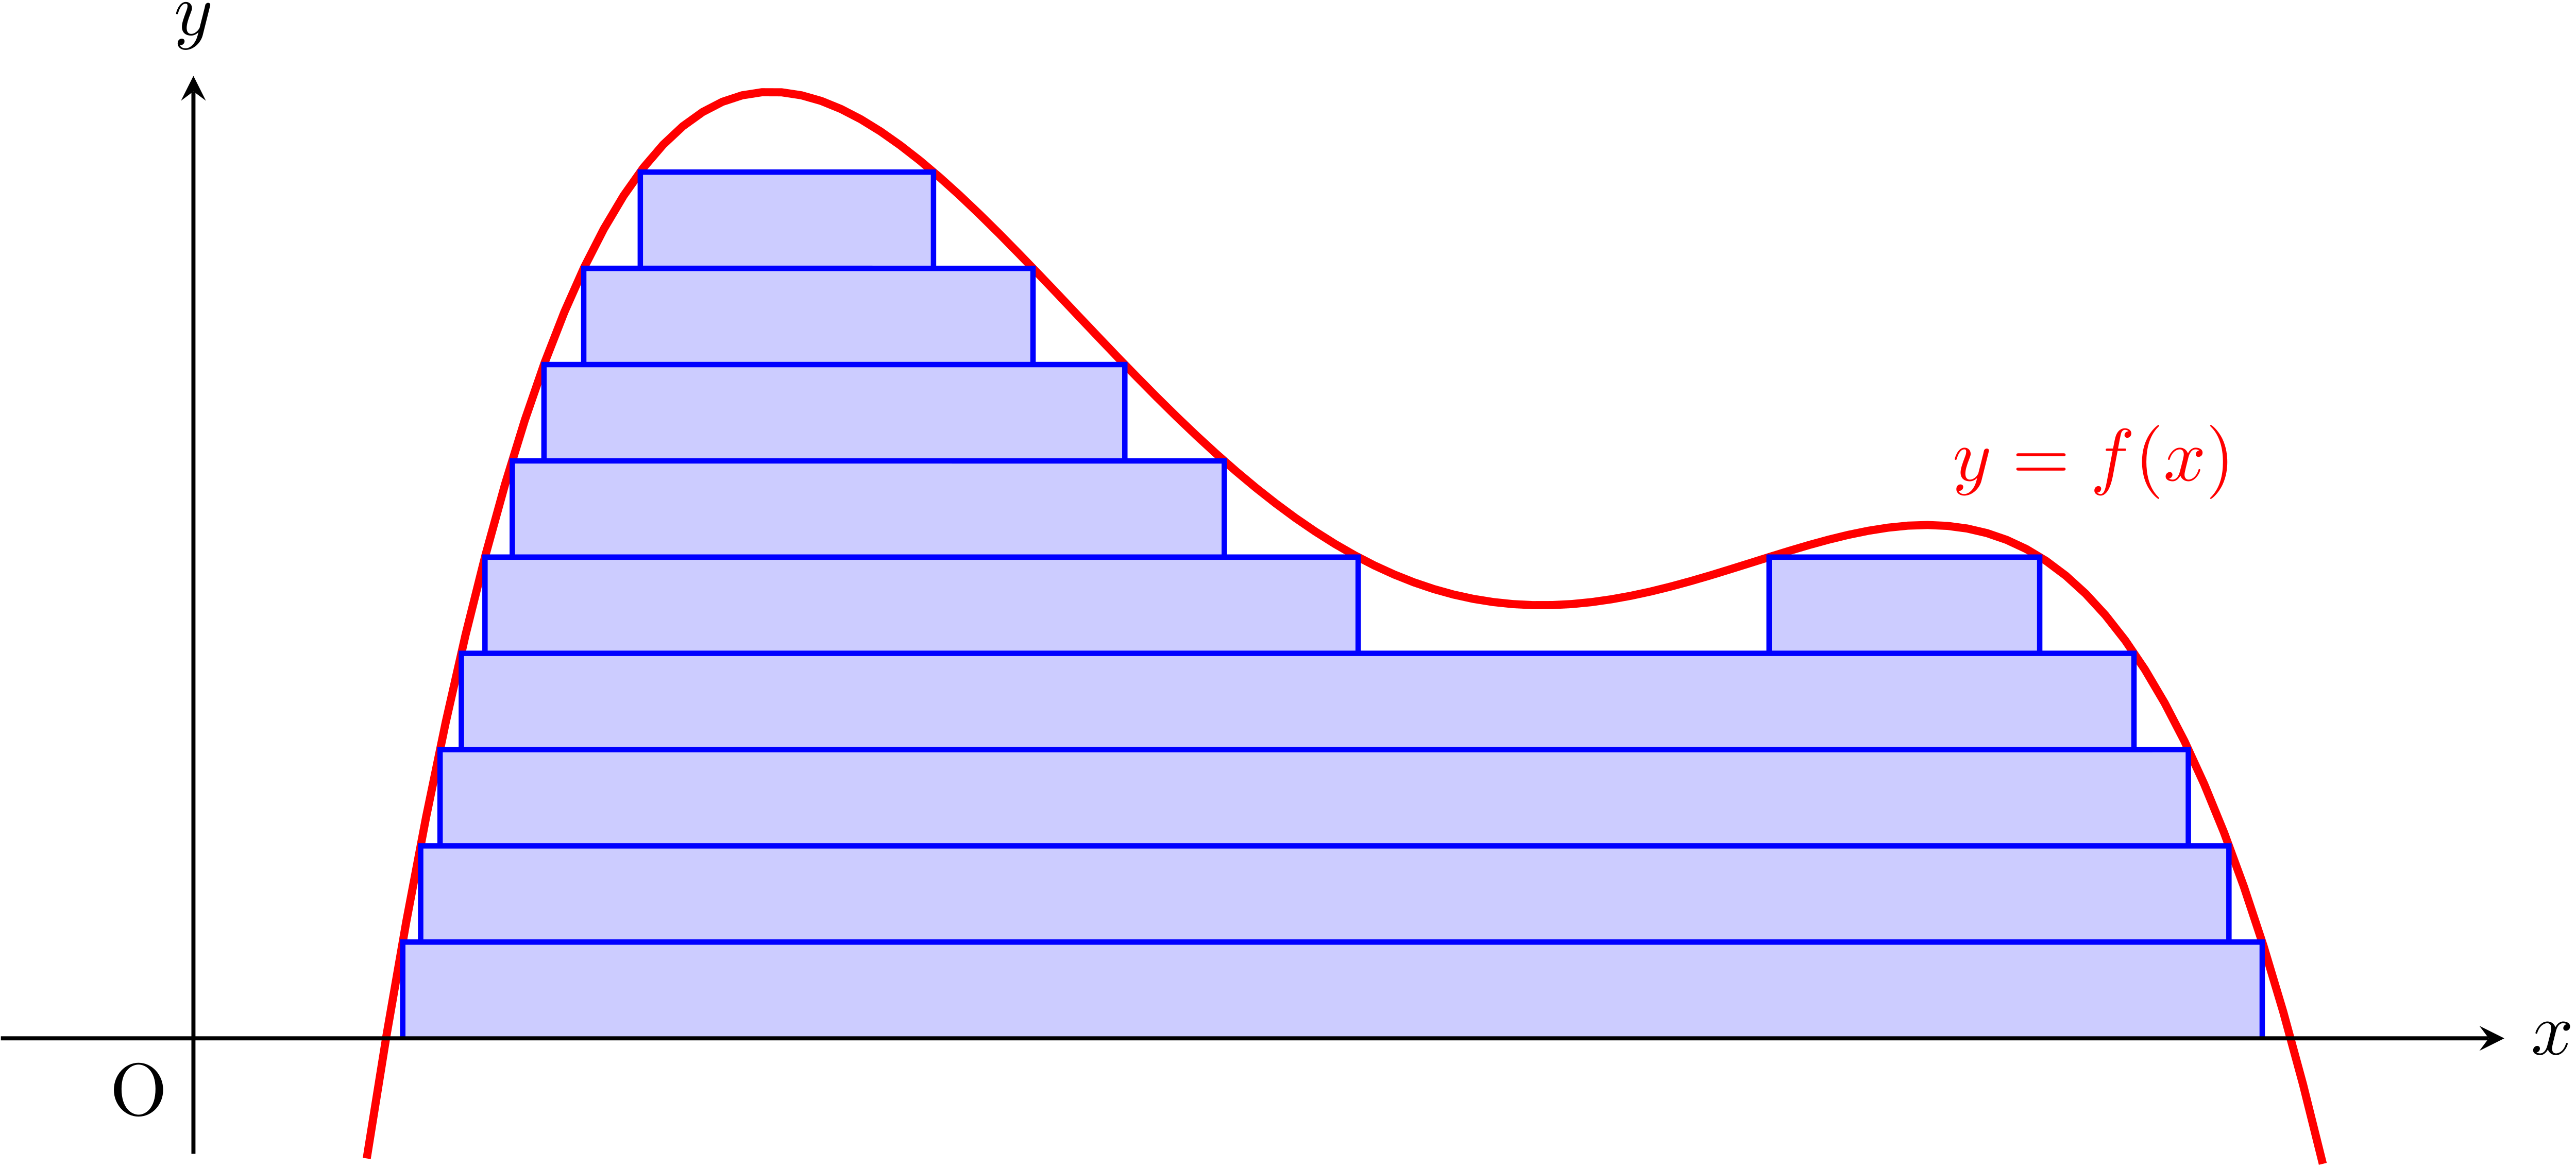
\includegraphics[scale=0.08]{figure/LI}
	\caption{Lebesgue积分示意图}
\end{figure}

\vskip 0.2cm
\begin{theorem}[非负可测简单函数积分的线性性]
	设$\varphi(x),\psi(x)$为$E \subset \R^n$上的非负可测简单函数, 
	$\alpha,\beta$为非负常数, 则有
	\begin{equation}
		\int_E (\alpha \varphi + \beta \psi) \d x = \alpha \int_E \varphi \d x + \beta \int_E \psi \d x.
	\end{equation}
\end{theorem}

\vskip 0.2cm
\begin{theorem}[非负可测简单函数积分的自可列可加性]
	设$\{ E_n \}_{n=1}^{\infty}$为递增可测集列, 
	$\varphi(x)$为$E = \bigcup\limits_{n=1}^{\infty} E_n$上的可测函数, 则
	\begin{equation}
		\lim\limits_{n\to\infty} \int_{E_n} \varphi(x) \d x = \int_E \varphi(x) \d x.
	\end{equation}
\end{theorem}

%%%%%%%%%%%%%%%%%%%%%%%%%%%%%%%%%%%%%%%%%%%%%%%%%%%%%%%%%%%%%%%%%%%%%%%%%%%%%%
%
%										下一小节
%
%%%%%%%%%%%%%%%%%%%%%%%%%%%%%%%%%%%%%%%%%%%%%%%%%%%%%%%%%%%%%%%%%%%%%%%%%%%%%%
\subsection{非负可测函数的Lebesgue积分}

\begin{definition}[非负可测函数的Lebesgue积分]
	设$E \subset \R^n$为可测集, $f(x)$为$E$上的一个非负可测函数, 定义$f(x)$在$E$上的Lebesgue积分为
	\begin{equation}
		\int_E f(x) \d x = \sup\limits_{\varphi \leq f \atop x\in E} 
		\left\{ \int_E \varphi(x) \d x : \varphi(x) \text{为} E \text{上的简单函数} \right\}.
	\end{equation}
	显然$0 \leq \int_E f(x) \d x \leq + \infty$, 
	若$\int_E f(x) \d x < \infty$, 则称$f(x)$在$E$上Lebesgue可积.
\end{definition}

\vskip 0.2cm
\begin{theorem}
	设$f(x),g(x)$为$E \subset \R^n$上的非负可测函数, $A$为$E$的可测子集, 则
	\begin{enumerate}
		\item 若$f \leq g$ a.e.于$E$, 则$\int_E f(x) \d x \leq \int_E g(x) \d x$; 这时若$g(x)$在$E$上可积, 则$f(x)$也在$E$上可积; 
		\item 若$\int_E f(x) \d x = 0$, 则$f(x) = 0$ a.e.于$E$;
		\item 若$\int_E f(x) \d x < \infty$, 则$0 \leq f(x) < \infty$ a.e.于$E$;
		\item $\int_A f(x) \d x = \int_E f(x) \cdot \chi_A \d x \leq \int_E f(x) \d x$. 
	\end{enumerate}
\end{theorem}
\begin{proof}\par 
	1.令$E_1 = E[f \leq g], E_2 = E[f > g]$, 则$E_1, E_2$都是$E$的可测子集, 且有
	$$
		E_1 \cup E_2 = E, \;
		E_1 \cap E_2 = \varnothing, \;
		m E_2 = 0 , 
	$$
	从而有
	$$
		\int_E f \d x = \int_{E_1} f \d x ,\;
		\int_E g \d x = \int_{E_1} g \d x .
	$$
	对于$E_1$上任一满足$\varphi(x) \leq f(x) \leq g(x)$的非负简单函数$\varphi(x)$,
	由定义有$\int_{E_1} \varphi \d x \leq \int_E g \d x = \int_{E_1} g \d x$.
	由此可得
	$$
		\int_{E_1} f(x) \d x = \sup\limits_{\varphi \leq f } 
		\left\{ \int_{E_1} \varphi(x) \d x \right\}
		\leq \int_{E_1} g(x) \d x .
	$$
	从而可知
	$$
		\int_E f(x) \d x \leq \int_E g(x) \d x.
	$$
	
	这时若$g(x)$在$E$上可积, 则
	$$
		\int_E f(x) \d x \leq \int_E g(x) \d x < \infty, 
	$$
	故$f(x)$也在$E$上可积
	\par  
	2. \framebox[\width]{截断法}\;
	对任意正整数$n$, 令
	$$
		\begin{aligned}
			A_n &= E\left[ f \geq \frac{1}{n} \right] ,\\
			\varphi_n(x) &= 
			\begin{cases}
				\frac 1n, & x \in A_n, \\
				0, & x \in E \backslash A_n.
			\end{cases}
		\end{aligned}
	$$
	则
	$$
		0 = \int_E f(x) \d x \geq \int_E \varphi_n(x) \d x = \frac 1n \cdot m A_n \geq 0.
	$$
	故$m A_n = 0, \forall n \in \N^*$. 
	而$E[f>0] = \bigcup\limits_{n=1}^{\infty} A_n$. 
	故$m E[f>0] = 0$, 因而$f(x) = 0$ a.e.于$E$.
	\par 
	3. \framebox[\width]{截断法}\;
	令$E_{\infty} = E[f = +\infty]$. 
	对任意正整数$n$, 令
	$$
		\varphi_n(x) = 
		\begin{cases}
			n, & x\in E_{\infty}, \\
			0, & x\in E \backslash E_{\infty}.
		\end{cases}
	$$
	则
	$$
		\infty > \int_E f(x) \d x \geq \int_E \varphi_n(x) \d x = n \cdot m E_{\infty} \geq 0.
	$$
	故
	$$
		0 \leq m E_{\infty} \leq \frac 1n \int_E f(x) \d x, \; \forall n \in \N^*.
	$$
	所以$m E_{\infty} = 0$, 即有$0 \leq f(x) < \infty$ a.e.于$E$
\end{proof}

\vskip 0.2cm
\begin{theorem}[Levi非负渐升列积分定理] \label{thm:Levi}
	设有定义在可测集$E \in \R^n$上的非负可测函数渐升列
	$$
		f_1(x) \leq f_2(x) \leq \cdots \leq f_k(x) \leq \cdots,
	$$
	令$f(x) = \lim\limits_{n \to \infty} f_n(x), x \in E$, 则
	\begin{equation}
		\lim\limits_{n \to \infty} \int_E  f_n(x) \d x = \int_E  f(x) \d x.
	\end{equation}
\end{theorem}
\begin{proof}
	显然有$f(x)$在$E$非负可测且$f_n(x) \leq f_{n+1}(x) \leq f(x)$, 故
	$$
		 \int_E  f_n(x) \d x \leq \int_E  f_{n+1}(x) \d x \leq \int_E  f(x) \d x.
	$$
	因而
	$$
		\lim\limits_{n \to \infty} \int_E  f_n(x) \d x \leq \int_E  f(x) \d x.
	$$
	下证相反的不等式. \par 
	任取$0<c<1$, 
	$\varphi(x)$为$E$上一简单非负函数, 满足$0 \leq \varphi(x) \leq f(x), \forall x \in E$. 
	记$E_n = E[f_n(x) \geq c\varphi] \subset E$, 显然有$E_n \subset E_{n+1}$, 
	且$\lim\limits_{n \to \infty} E_n = \bigcup\limits_{n=1}^{\infty} E_n = E$, 于是有不等式
	$$
		\int_E f_n(x) \d x \geq \int_{E_n} f_n(x) \d x \geq \int_{E_n} c \varphi(x) \d x = c\int_{E_n} \varphi(x) \d x.
	$$
	根据非负简单函数积分的自可列可加性, 可知
	$$
		\lim\limits_{n \to \infty} \int_{E_n} \varphi(x) \d x = \int_E \varphi(x) \d x .
	$$
	综上我们得到
	$$
		\lim\limits_{n \to \infty} \int_E f_n(x) \d x \geq c \int_E \varphi(x) \d x .
	$$
	上式中令$c \to 1$, 有
	$$
		\lim\limits_{n \to \infty} \int_E f_n(x) \d x \geq \int_E \varphi(x) \d x .
	$$
	再由非负可测函数积分的定义, 有
	$$
		\lim\limits_{n \to \infty} \int_E  f_n(x) \d x \geq \int_E  f(x) \d x.
	$$
\end{proof}

上述定理表明, 对于非负可测函数渐升列来说, 极限与积分的次序可以交换. 
此外, 由于非负可测函数是非负可测简单函数渐升列的极限, 因而使得积分理论中的许多结果可直接从可测简单函数的积分性质得到. 

\vskip 0.2cm
\begin{theorem}[非负可测函数积分的线性性]
	设$f(x),g(x)$为$E \subset \R^n$上的非负可测函数, 
	$\alpha,\beta$为非负常数, 则有
	\begin{equation}
		 \int_E (\alpha f + \beta g) \d x = \alpha \int_E f \d x + \beta \int_E g \d x.
	\end{equation}
\end{theorem}

\vskip 0.2cm
\begin{theorem}[逐项积分定理]
\label{thm:Progressive Integral}
	设$\{ f_n (x) \}$是E上的非负可测函数列, 则
	\begin{equation}
		\int_E \left( \sum\limits_{n = 1}^{\infty} f_n(x) \right) \d x
		= \sum\limits_{n = 1}^{\infty} \int_E f_n(x) \d x.
	\end{equation}
\end{theorem}
\begin{proof}
	令$S_n (x) = \sum\limits_{k = 1}^{n} f_k(x)$, 
	则$\{ S_n(x) \}$为$E$上非负可测函数渐升列. 
	从而根据Levi非负渐升列积分定理(Thm:\ref{thm:Levi})以及积分的线性性质, 可知
	$$
	\begin{aligned}
		\int_E \left( \sum\limits_{n = 1}^{\infty} f_n(x) \right) \d x
		& = \int_E \left(\lim\limits_{n \to \infty} S_n(x)  \right) \d x 
		 = \lim\limits_{n \to \infty} \int_E S_n(x) \d x \\
		& = \lim\limits_{n \to \infty} \sum\limits_{k = 1}^{n} \int_E f_n(x) \d x
		 = \sum\limits_{n = 1}^{\infty} \int_E f_n(x) \d x.
	\end{aligned}
	$$
\end{proof}

\vskip 0.2cm
\begin{theorem}[Fatou引理]
	设$\{ f_n (x) \}$是$E$上的非负可测函数列, 则
	\begin{equation}
		\int_E \varliminf\limits_{n \to \infty} f_n(x) \d x \leq 
		\varliminf\limits_{n \to \infty} \int_E f_n(x) \d x .
	\end{equation}
\end{theorem}
\begin{proof}
	令$g_n (x) = \inf \{ f_k(x) : k \geq n \}$, 
	则$\{ g_n(x) \}$为$E$上的非负可测渐升函数列, 且$x \in E$时有
	$$
		0 \leq g_n(x) \leq g_{n+1}(x) \leq f_{n+1}(x).
	$$
	从而由Levi非负渐升列积分定理(Thm:\ref{thm:Levi})
	$$
		\int_E \varliminf\limits_{n \to \infty} f_n(x) \d x
		= \int_E \lim\limits_{n \to \infty} g_n(x) \d x
		= \lim\limits_{n \to \infty} \int_E g_n(x) \d x
		\leq \varliminf\limits_{n \to \infty} \int_E f_n(x) \d x .
	$$
\end{proof}
\vskip 0.4cm
Fatou引理常用于判断极限函数的可积性. 
例如, 当$E$上的非负可测函数列$\{ f_n (x) \}$满足
$$
	\int_E f_k(x) \d x \leq M \quad k=1,2,\cdots
$$
时, 我们就得到
$$
	\int_E \varliminf\limits_{n \to \infty} f_n(x) \d x \leq M .
$$

下面的例子说明Fatou引理中的不等号是可能成立的. 

\begin{example}
	在$[0,1]$上作非负可测函数列
	$$
	f_n(x) = 
	\begin{cases}
		0, & x=0, \\
		n, & 0 < x < \frac{1}{n}, \\
		0, & \frac{1}{n} < x <1,
	\end{cases}
	\quad n = 1,2,\cdots
	$$
	显然有$\lim\limits_{n \to \infty} f_n(x) = 0 \;(x \in [0,1]).$
	因此
	$$
		\int_{[0,1]} \varliminf\limits_{n \to \infty} f_n(x) \d x = 0 
		< 
		1 = \varliminf\limits_{n \to \infty} \int_{[0,1]} f_n(x) \d x .
	$$
\end{example}




%%%%%%%%%%%%%%%%%%%%%%%%%%%%%%%%%%%%%%%%%%%%%%%%%%%%%%%%%%%%%%%%%%%%%%%%%%%%%%
%
%										下一小节
%
%%%%%%%%%%%%%%%%%%%%%%%%%%%%%%%%%%%%%%%%%%%%%%%%%%%%%%%%%%%%%%%%%%%%%%%%%%%%%%
\subsection{一般可测函数的Lebesgue积分}

\begin{definition}[一般可测函数的Lebesgue积分]
	设$f(x)$为$E \subset \R^n$上的可测函数, 若积分
	$$
		\int_E f^+ (x) \d x, \;
		\int_E f^- (x) \d x
	$$
	中至少有一个是有限值, 则称$f$在$E$上的\textbf{积分确定}, 称
	$$
		\int_E f (x) \d x = \int_E f^+ (x) \d x - \int_E f^- (x) \d x
	$$
	为$f$在$E$上的\textbf{Lebesgue积分}; 
	当上式右端两个积分值皆为有限时, 则称$f$在$E$上是\textbf{可积}的. 
	在$E$上可积的函数的全体记为$L(E)$.
\end{definition}

由于$\int_E |f (x)| \d x = \int_E f^+ (x) \d x + \int_E f^- (x) \d x$, 
故知在$f$可测的条件下, $f(x)$的可积性与$| f(x) |$的可积性是等价的. 
此时还有$|\int_E f \d x| \leq \int_E |f| \d x$. 


\begin{theorem}[$L$积分的一些基本性质]
	\begin{enumerate}
		\item (零测集上实函数$L$可积) \\
		\quad  若$E \neq \varnothing$但$mE=0$, 则$E$上的任何实函数$f$都在$E$上$L$可积且
			$$
				\int_E f \d x = 0;
			$$
		\vskip 0.2cm
		\item ($L$可积函数几乎处处有限) \\
		\quad  若$f \in L(E)$, 则$m E[|f| = \infty] = 0$, 即$|f(x)| < \infty$ a.e.于$E$; 
		\vskip 0.2cm
		\item ($L$积分定义域具有可加性) \\
		\quad 设$f$在可测集$A,B$上积分确定, 且$A \cap B = \varnothing$, 那么
		$$
			\int_{A \cup B} f(x) \d x = \int_{A} f(x) \d x+\int_{B} f(x) \d x ;
		$$
		\vskip 0.2cm
		\item (a.e.相等的函数的$L$积分a.e.相等) \\
		\quad 设$f$在$E$上积分确定, 且$f(x)=g(x)$ a.e.于$E$, 那么$g$也在$E$上积分确定且
		$$
			\int_{E} f(x) \d x = \int_{E} g(x) \d x .
		$$
		特别的, 若$mE < \infty$且$b \leq f(x) \leq B$ a.e.于E, 则
		$$
			bmE \leq \int_E f(x) \d x \leq BmE;
		$$
		\vskip 0.2cm
		\item ($L$积分的保序性) \\
		\quad 设$f, g$在$E$上积分确定, 且$f(x) \leq g(x)$ a.e.于$E$, 那么
		$$
			\int_{E} f(x) \d x \leq \int_{E} g(x) \d x ;
		$$
		\vskip 0.2cm
		\item ($L$积分的绝对值小于等于绝对值的$L$积分)\\
		\quad 设$f$在$E$上$L$可积, 则$|f|$在$E$上亦$L$可积, 且
		$$
			\left|\int_{E} f(x) \d x \right| \leq \int_{E} |f(x)| \d x ;
		$$
		\vskip 0.2cm
		\item (控制可积) \\
		\quad 设$f$在$E$上可测, $g$是$E$上的非负$L$可积函数且$|f(x)| \leq g(x)$ a.e.于$E$, 则$f$在$E$上$L$可积且
		$$
			\left|\int_{E} f(x) \d x \right| \leq \int_{E} |f(x)| \d x \leq \int_{E} g(x) \d x. 
		$$
		一般我们称$g(x)$为$f(x)$的控制函数. 
	\end{enumerate}
\end{theorem}

\vskip 0.2cm
\begin{theorem}[$L$积分的线性性]
	设$f(x),g(x)$为$E \subset \R^n$上的$L$可积函数, 
	对任意$\alpha,\beta \in \R$, 有
	\begin{equation}
		 \int_E (\alpha f + \beta g) \d x = \alpha \int_E f \d x + \beta \int_E g \d x.
	\end{equation}
\end{theorem}

\vskip 0.2cm
\begin{theorem}[$L$积分的绝对连续性]
	设$f$为$E$上可积函数, 则对任意$\varepsilon > 0$, 存在$\delta > 0$, 
	使得对于任意$E$的可测子集$A$满足$mA < \delta$时, 有
	\begin{equation}
		\left| \int_A f(x) \d x \right| \leq \int_A |f(x)| \d x < \varepsilon.
	\end{equation}
\end{theorem}
\begin{proof}
	由于$f \in L(E)$, 故$|f(x)| \in L(E)$. 
	由Riesz表示定理(Thm:\ref{thm:Riesz1}), 对于任意$\varepsilon > 0$, 
	存在$E$上的简单函数满足$0 \leq \varphi(x) \leq |f(x)|$, 且
	$$
		\int_E |f(x)| \d x - \frac{\varepsilon}{2} 
		\leq \int_E \varphi(x) \d x
		\leq \int_E |f(x)| \d x.
	$$
	令$M = \max \{ \varphi(x): x \in E \}$, 
	$\delta = \frac{\varepsilon}{1 + 2M}$, 
	则对于任何可测集$A \subset E$, 只要有$mA < \delta$, 就有
	$$
	\begin{aligned}
		\left| \int_A f(x) \d x \right| 
		&\leq \int_A |f(x)| \d x \\
		&= \int_A (|f(x)| - \varphi(x)) \d x + \int_A \varphi(x) \d x \\
		&\leq \frac{\varepsilon}{2} + M \cdot mA \\
		&< \frac{\varepsilon}{2} + M \cdot \frac{\varepsilon}{1 + 2M} 
		< \varepsilon. 
	\end{aligned}
	$$
\end{proof}

\begin{theorem}[$L$积分对定义域的可数可加性]
	设可测子集列$\{ E_n \}$满足$E_i \cap E_j = \varnothing \; (i \neq j)$. 
	$f$在$E = \bigcup\limits_{n = 1}^{\infty} E_n$上积分确定, 则
	\begin{equation}
		\int_E f(x) \d x = \sum\limits_{n = 1}^{\infty} \int_{E_n} f(x) \d x.
	\end{equation}
\end{theorem}
\begin{proof}
	对任意$n \in \N^*$, 
	令$f_n = f^+ \cdot \chi_{E_n}, g_n = f^- \cdot \chi_{E_n}$, 则
	$$
		f^+(x) = \sum\limits_{n = 1}^{\infty} f_n(x) , \;
		f^-(x) = \sum\limits_{n = 1}^{\infty} g_n(x) . 
	$$
	由逐项积分定理(Thm:\ref{thm:Progressive Integral})
	$$
	\begin{aligned}
		\int_E f(x) \d x
		&= \int_E f^+(x) \d x - \int_E f^-(x) \d x \\
		&= \int_E \sum\limits_{n = 1}^{\infty} f_n(x) \d x 
			- \int_E \sum\limits_{n = 1}^{\infty} g_n(x) \d x \\
		&= \sum\limits_{n = 1}^{\infty} \int_{E_n} f^+(x) \chi_{E_n} \d x
			- \sum\limits_{n = 1}^{\infty} \int_{E_n} f^-(x) \chi_{E_n} \d x \\
		&= \sum\limits_{n = 1}^{\infty} \int_{E_n} f^+(x) \d x
			- \sum\limits_{n = 1}^{\infty} \int_{E_n} f^-(x) \d x \\
		&= \sum\limits_{n = 1}^{\infty} \int_{E_n} (f^+(x) - f^-(x)) \d x
	\end{aligned}
	$$
\end{proof}



\begin{theorem}[积分变量的平移变换定理]
	若$f \in L( E )$, 则对任意的$x_0 \in E, \; f(x+x_0) \in L( E )$, 有
	\begin{equation}
		\int_E f(x + x_0) \d x = \int_E f(x) \d x.
	\end{equation}
\end{theorem}
\begin{proof}
	只需考虑$f \geq 0$的情形. 
	首先考虑$f$为非负可测简单函数:
	$$
		f(x) = \sum\limits_{i=1}^n c_i \chi_{E_i}(x) , \; x\in E. 
	$$
	显然有
	$$
		f(x + x_0) = \sum\limits_{i=1}^n c_i \chi_{E_i - \{x_0\}}(x) , \; x\in E
	$$
	仍为非负可测简单函数,从而
	$$
	\begin{aligned}
		\int_E f(x + y_0) \d x &= 
		\sum\limits_{i=1}^n c_i m( E_i - \{x_0\} ) \\
		&= \sum\limits_{i=1}^n c_i m( E_i ) = \int_E f(x) \d x.
	\end{aligned}
	$$
	
	其次, 考虑一般非负可测函数$f(X)$. 
	此时存在非负可测简单函数渐升列$\{ \varphi_n (x) \}$, 使得$\lim\limits_{n \to \infty} \varphi_n (x) = f(x), \; x \in E$. 
	显然$\{ \varphi_n (x + x_0) \}$仍为渐升列, 且有
	$$
		\lim\limits_{n \to \infty} \varphi_n (x + x_0) = f(x + x_0), \; x \in E.
	$$
	从而
	$$
	\begin{aligned}
		\int_E f(x + y_0) \d x &= 
		\lim\limits_{n \to \infty} \int_E \varphi_n (x + y_0) \d x \\
		&= \lim\limits_{n \to \infty} \int_E \varphi_n (x)\d x = \int_E f(x) \d x.
	\end{aligned}
	$$
\end{proof}

\begin{definition}[平均收敛]
	设$\{ f_n(x) \}$为$E$上的可积函数列, $f(x)$在$E$上可积, 若
	$$
		\lim\limits_{n \to \infty} \int_E |f_n -f| \d x = 0,
	$$
	则称$\{ f_n(x) \}$(1次幂)\textbf{平均收敛}于$f(x)$.
\end{definition}

\begin{theorem}[平均收敛一定依测度收敛]
	设$\{ f_n(x) \}$为$E$上的可积函数列, $f(x)$在$E$上可积, 若
	$$
		\lim\limits_{n \to \infty} \int_E |f_n -f| \d x = 0,
	$$
	那么有$\{ f_n(x) \}$依测度收敛于$f(x)$. 
\end{theorem}

\begin{proof}
	\framebox[\width]{截断法}\;
	对任意$\sigma > 0$, 记$E_n = E[|f_n - f| \geq \sigma]$, 由
	$$
	\begin{aligned}
		\sigma m E_n 
		&= \int_{E_n} \sigma \d x 
		\leq \int_{E_n} |f_n - f| \d x \\
		&\leq \int_E |f_n - f| \d x \to 0 \quad (n \to \infty)
	\end{aligned}
	$$
	所以有$\lim\limits_{n \to \infty} m E_n = 0$. 
\end{proof}

进一步地, 由Riesz定理(Thm:\ref{thm:Riesz2}), 存在子列$\{ f_{n_j}(x) \}$使得
$$
	\lim\limits_{j \to \infty} f_{n_j}(x) = f(x) \quad \text{a.e.} x \in E.
$$

\begin{proposition}[闭区间上存在连续函数平均收敛于$L$可积函数]
	设$f \in L[a,b]$, 则对于任意$\varepsilon >0$, 存在$g \in C[a,b]$, 使得
	$$
		\int_{[a,b]} |f(x) - g(x)| < \varepsilon.
	$$
\end{proposition}
\begin{proof}  
\framebox[\width]{简单函数$\varphi(x)$逼近$f(x)$} \par 
由于$f \in L[a, b]$, 故$f^+$和$f^-$都在$[a, b]$上非负$L$可积.
对于任意的$\varepsilon>0$, 存在$[a, b]$上的两个非负简单函数$\varphi_{1}$和$\varphi_{2}$, 
使得$x \in[a, b]$时, $0 \leq \varphi_1 (x) \leq f^+(x), 0 \leq \varphi_2 (x) \leq f^-(x)$. 且
$$
\begin{array}{l}
\int_{[a, b]} f^+(x) \d x-\frac{\varepsilon}{4} \leq \int_{[a, b]} \varphi_1 (x) \d x \leq \int_{[a, b]} f^+(x) \d x \\
\int_{[a, b]} f^-(x) \d x-\frac{\varepsilon}{4} \leq \int_{[a, b]} \varphi_2 (x) \d x \leq \int_{[a, b]} f^-(x) \d x
\end{array}
$$
令$\varphi(x)=\varphi_1 (x)-\varphi_2 (x)$, 
则$\varphi$是$[a, b]$上的简单函数, 且
$$
\begin{aligned}
\int_{[a, b]}|f(x)-\varphi(x)| \d x &=\int_{[a, b]}\left|f^+(x)-f^-(x)-\varphi_1 (x)+\varphi_2 (x)\right| \d x \\
& \leq \int_{[a, b]}\left|f^+(x)-\varphi_1 (x)\right| \d x+\int_{[a, b]}\left|f^-(x)-\varphi_2 (x)\right| \d x \\
&=\left(\int_{[a, b]} f^+(x) \d x-\int_{[a, b]} \varphi_1 (x) \d x\right)+\left(\int_{[a, b]} f^-(x) \d x-\int_{[a, b]} \varphi_2 (x) \d x\right) \\
& \leq \frac{\varepsilon}{4}+\frac{\varepsilon}{4}=\frac{\varepsilon}{2}.
\end{aligned}
$$ 

\framebox[\width]{根据Лузин定理', 此处直接写出$g$存在性即可} \par
令 $M=\max \{|\varphi(x)|: x \in[a, b]\}$, 
令 $\delta=\frac{\varepsilon}{1+4 M}$, 
由Лузин定理'(Thm:\ref{thm:Lusin2}), 
存在闭集$F \subset[a, b]$满足$m([a, b] \backslash F)<\delta$
以及$g \in C[a, b]$, 使得对任意$x \in F$, 有$g(x)=\varphi(x)$; 
且$x \in[a, b]$时, 有$|g(x)| \leq M$. 
于是
$$
\begin{aligned}
	\int_{[a, b]}|\varphi(x)-g(x)| \d x
	&= \int_{[a, b] \backslash F}|\varphi(x)-g(x)| \d x \\
	&\leq \int_{[a, b] \backslash F}|\varphi(x)| \d x - \int_{[a, b] \backslash F}|g(x)| \d x \\
	&< M \delta + M \delta < \frac{\varepsilon}{2}.
\end{aligned}
$$
因而
$$
\begin{aligned}
	     & \int_{[a,b]} |f(x) - g(x)| \d x \\
	\leq & \int_{[a, b]}|f(x)-\varphi(x)| \d x + \int_{[a, b]}|\varphi(x)-g(x)| \d x \\
	<    & \frac{\varepsilon}{2} + \frac{\varepsilon}{2} = \varepsilon.
\end{aligned}
$$
\end{proof}


































%%%%%%%%%%%%%%%%%%%%%%%%%%%%%%%%%%%%%%%%%%%%%%%%%%%%%%%%%%%%%%%%%%%%%%%%%%%%%%
%
%										下一节
%
%%%%%%%%%%%%%%%%%%%%%%%%%%%%%%%%%%%%%%%%%%%%%%%%%%%%%%%%%%%%%%%%%%%%%%%%%%%%%%
\section{积分收敛定理}

控制收敛定理的直接结论是平均收敛, 为积分与极限次序的交换所提供的了充分条件. 
它是Lebesgue积分理论中最重要的结果之一.

\begin{theorem}[Lebesgue控制收敛定理]\label{thm:Ldc}
	设$\{ f_n(x) \}_{n=1}^{\infty}$为$E$上的可测函数列, 且有
	$$
		\lim\limits_{n \to \infty} f_n(x) = f(x), \; a.e. x \in E.
	$$
	若存在$E$上的可积函数$F(x)$, 使得对任意的$n \in \N^*$
	$$
		|f_n(x)| \leq F(x), \; a.e. x \in E ,
	$$
	则
	\begin{enumerate}
		\item 
		\begin{equation}
			\lim\limits_{n\to\infty}\int_E |f_n(x) - f(x)| \d x = 0,
		\end{equation}
		
		\item 
		\begin{equation}
			\lim\limits_{n\to\infty}\int_E f_n(x) \d x = \int_E f(x)\d x.
		\end{equation}
	\end{enumerate}
	
	(通常称$F(x)$为函数列$\{ f_n(x) \}$的\textbf{控制函数}.)
\end{theorem}
\begin{proof} 
	\framebox[\width]{记$g_n(x) = |f_n(x) - f(x)|$} \par 
	显然$f$在$E$上可测且$|f(x)| \leq F(x) \;\text{a.e.} x\in E$. 
	从而$f(x)$, 每个$f_n(x)$均可积. 
	
	令$g_n(x) = |f_n(x) - f(x)|$, 则$g(x)$在$E$上可积且满足
	$$
	\begin{aligned}
		& 0 \leq g_n(x) \leq |f_n(x)| + |f(x)| \leq 2F(x), \\ 
		& \lim\limits_{n \to \infty} g_n(x) = 0, 
	\end{aligned}
		 \quad a.e. x \in E.
	$$
	从而有
	$$
	\begin{aligned}
		& 2F(x) - g_n(x) \geq 0, \\ 
		& \lim\limits_{n \to \infty} 2F(x) - g_n(x) = 2F(x), 
	\end{aligned}
		 \quad a.e. x \in E.
	$$
	\framebox[\width]{由Fatou引理"压平"$g_n(x)$} \par
	由Fatou引理
	$$
	\begin{aligned}
		2 \int_E F(x) \d x
		&= \int_E \lim\limits_{n \to \infty} (2F(x) - g_n(x)) \d x \\
		&\leq \varliminf\limits_{n \to \infty} \int_E (2F(x) - g_n(x)) \d x \\
		&= 2 \int_E F(x) \d x + \varliminf\limits_{n \to \infty} \left(- \int_E g_n(x) \d x \right) \\
		&= 2 \int_E F(x) \d x - \varlimsup\limits_{n \to \infty} \int_E g_n(x) \d x.
	\end{aligned}
	$$
	故$\varlimsup\limits_{n \to \infty} \int_E g_n(x) \d x \leq 0$,
	又$\int_E g_n(x) \d x \geq 0$, 
	从而$\lim\limits_{n \to \infty} \int_E g_n(x) \d x = 0$, 
	即
	$$
		\lim\limits_{n \to \infty} \int_E |f_n(x) - f(x)| \d x = 0.
	$$
	从而
	$$
		0 \leq 
		\lim\limits_{n \to \infty} \left| \int_E f_n(x) \d x - \int_E f(x) \d x \right|
		\leq \lim\limits_{n \to \infty} \int_E |f_n(x) - f(x)| \d x = 0
	$$
\end{proof}

\begin{theorem}[依测度收敛型Lebesgue控制收敛定理]
	设$\{ f_n(x) \}_{n=1}^{\infty}$为$E$上的可测函数列, 
	且$f_n(x)$在$E$上依测度收敛于$f(x)$. 
	若存在$E$上的可积函数$F(x)$, 使得对任意的$n \in \N^*$
	$$
		|f_n(x)| \leq F(x), \; a.e. x \in E ,
	$$
	则
	\begin{enumerate}
		\item 
		\begin{equation}
			\lim\limits_{n\to\infty}\int_E |f_n(x) - f(x)| \d x = 0,
		\end{equation}
		
		\item 
		\begin{equation}
			\lim\limits_{n\to\infty}\int_E f_n(x) \d x = \int_E f(x)\d x.
		\end{equation}
	\end{enumerate}
\end{theorem}
\begin{proof}
	反证法. 
	设有$\lim\limits_{n \to \infty}\int_E |f_n(x) - f(x)| \d x \neq 0$, 
	则存在$\{ f_n \}$的子列$\{ f_{n_j} \}$使得
	$$
	\begin{array}{c r}
		\lim\limits_{j\to\infty}\int_E |f_{n_j}(x) - f(x)| \d x = \alpha >0. 
		&  (*)
	\end{array}
	$$
	又$\{ f_{n_j} \}$依测度收敛于$f(x)$, 根据Riesz定理(Thm:\ref{thm:Riesz2}), 
	存在$\{ f_{n_j} \}$的子列$\{ f_{n_{j_k}} \}$使得
	$$
		\lim\limits_{k\to\infty}  f_{n_{j_k}}(x) = f(x),\;\text{a.e.} x\in E.
	$$
	由Lebesgue控制收敛定理(Thm:\ref{thm:Ldc}), 
	$$
		\lim\limits_{k\to\infty}\int_E |f_{n_{j_k}}(x) - f(x)| \d x = 0.
	$$
	这与($*$)式相矛盾, 故
	$$
		\lim\limits_{n\to\infty}\int_E |f_n(x) - f(x)| \d x = 0.
	$$
\end{proof}

\begin{corollary}
	设$E \subset \R^n$为可测集, $m E < \infty$, $f$和$f_n\;(n=1,2,\cdots)$都是$E$上的可测函数. 
	如果存在$M > 0$使得对于任意的正整数$n$, $| f_n | \leq M$ a.e.$x \in E$, 且$n \to \infty$时有
	$$
		f_n(x) \to f(x) \;\text{a.e.} x \in E
		\text{或}
		f_n(x) \text{依测度收敛于} f, 
	$$
	则
	\begin{enumerate}
		\item 
		\begin{equation}
			\lim\limits_{n\to\infty}\int_E |f_n(x) - f(x)| \d x = 0,
		\end{equation}
		
		\item 
		\begin{equation}
			\lim\limits_{n\to\infty}\int_E f_n(x) \d x = \int_E f(x)\d x.
		\end{equation}
	\end{enumerate}	
\end{corollary}

\begin{theorem}[逐项积分定理]
	设$\{ f_n(x) \}_{n=1}^{\infty}$为$E$上的$L$可积函数列, 如果正项级数$\sum\limits_{n = 1}^{\infty} \int_E | f_n(x) | \d x$收敛, 则函数项级数$\sum\limits_{n = 1}^{\infty} f_n(x)$在$E$上a.e.收敛, 其和函数在$E$上$L$可积且
	\begin{equation}
		\int_E \sum\limits_{n = 1}^{\infty} f_n(x) \d x =
		\sum\limits_{n = 1}^{\infty} \int_E f_n(x) \d x.
	\end{equation}
\end{theorem}
\begin{proof}
	令
	$$
		F(x) = \sum\limits_{n = 1}^{\infty} |f_n(x)|, \; x \in E.
	$$
	由逐项积分定理(Thm:\ref{thm:Progressive Integral})
	$$
		\int_E F(x) \d x
		= \int_E \sum\limits_{n = 1}^{\infty} |f_n(x)| \d x
		= \sum\limits_{n = 1}^{\infty} \int_E |f_n(x)| \d x
		< \infty.
	$$
	故$F(x)$在$E$上非负$L$可积, 所以$0 \leq F(x) < \infty$ a.e.$x \in E$, 
	因而$\sum\limits_{n = 1}^{\infty} f_n(x)$在$E$上 a.e.收敛. 
	
	令
	$$
		g(x) = \sum\limits_{n = 1}^{\infty} f_n(x) ,\quad
		g_n(x) = \sum\limits_{k = 1}^{n} f_k(x) ,\quad
		x \in E ,
	$$
	则
	$$
		| g_n(x) | \leq \sum\limits_{k = 1}^{n} | f_k(x) | \leq F(x) 
		\;\text{a.e.} x \in E
	$$
	且$n \to \infty$时, $g_n(x) \to g(x)$ a.e.于$E$, 
	由Lebesgue控制收敛定理(Thm:\ref{thm:Ldc}), $g$在$E$上$L$可积且
	$$
		\begin{aligned}
			\int_E g(x) \d x
			&= \lim\limits_{n \to \infty} \int_E g_n(x) \d x \\
			&= \lim\limits_{n \to \infty} \int_E \sum\limits_{k = 1}^{n} f_k(x) \d x 
			= \lim\limits_{n \to \infty}  \sum\limits_{k = 1}^{n} \int_E f_k(x) \d x \\
			&= \sum\limits_{n = 1}^{\infty} \int_E f_n(x) \d x \; ,
		\end{aligned}
	$$
	即
	$$
		\int_E \sum\limits_{n = 1}^{\infty} f_n(x) \d x =
		\sum\limits_{n = 1}^{\infty} \int_E f_n(x) \d x.
	$$
\end{proof}

\begin{theorem}[积分号下求导]
	设$E \subset \R^n$为可测集, $f(x, t)$为$E \times (a, b)$上的实函数. 
	如果对任意$t_0 \in (a, b)$, $f(x, t_0)$在$E$上$L$可积; 
	对于 a.e.的$x_0 \in E$, $f(x.t)$作为$t$的函数在$(a, b)$上可导且存在
	$\left| \frac{\partial}{\partial t} f(x, t) \right| \leq F(x_0)$, 
	此处的$F$为$E$上某个非负$L$可积函数, 则$\int_E f(x,t) \d x$在$(a,b)$上可导且
	\begin{equation}
		\frac{\d}{\d t} \int_E f(x, t) \d x = \int_E \frac{\partial}{\partial t} f(x, t) \d x.
	\end{equation}
\end{theorem}
\begin{proof}
	任意取定$t \in (a, b)$以及$h_n \to 0 \; (n \to \infty)$, 我们有
	$$
		\lim\limits_{n \to \infty} \frac{f(x, t+h_n) - f(x, t)}{h_n}
		= \frac{\partial}{\partial t} f(x, t), \; x\in E.
	$$
	且当$k$充分大时, 由微分中值定理, 有下式成立
	$$
		\left| \frac{f(x, t+h_n) - f(x, t)}{h_n} \right|
		= \left| \frac{\partial}{\partial t} f(x, t + \theta_n h_n ) \right|
		\leq F(x) \; \text{a.e.} \; x\in E,
	$$
	其中$0 < \theta_n <1$, 从而由Lebesgue控制收敛定理(Thm:\ref{thm:Ldc})可得
	$$
		\frac{\d}{\d t} \int_E f(x, t) \d x
		= \lim\limits_{n \to \infty} \frac{1}{h_n} \int_E [ f(x, t+h_n) - f(x, t) ] \d x
		= \int_E \lim\limits_{n \to \infty} \frac{f(x, t+h_n) - f(x, t)}{h_n} \d x
		= \int_E \frac{\partial}{\partial t} f(x, t) \d x.
	$$
\end{proof}
%\begin{center}
%\begin{tikzpicture}
%
%	\tikzstyle{every node}=[font=\small,scale=1] %放大
%
%	\node[draw, rounded corners]                       (LC1)   {Lebesgue控制收敛定理};
%	\node[draw, rounded corners, right = 20pt of LC1]  (LC2)  {依测度收敛型Lebesgue控制收敛定理};
%	\node[draw, rounded corners, right = 20pt of LC2] (Levi)   {Levi 非负渐升列积分定理};
%	
%	\tikzstyle{arrow1} = [thick,<->,>=stealth]
%	\draw[arrow1] (LC1)       --    (LC2);
%	\tikzstyle{arrow2} = [thick,->,>=stealth]
%	\draw[arrow2] (LC2)       --    (Levi);
%	
%\end{tikzpicture}	
%\end{center}
%\vskip 0.5cm
%%%%%%%%%%%%%%%%%%%%%%%%%%%%%%%%%%%%%%%%%%%%%%%%%%%%%%%%%%%%%%%%%%%%%%%%%%%%%%
%
%										下一节
%
%%%%%%%%%%%%%%%%%%%%%%%%%%%%%%%%%%%%%%%%%%%%%%%%%%%%%%%%%%%%%%%%%%%%%%%%%%%%%%
\section{Riemann积分与Lebesgue积分}

至此,我们已经基本上建立了Lebesgue积分理论, 在进一步介绍这一理论的其他内容以前, 我们先来揭示它与Riemann积分的关系. 
这一关系可以用一个公式来表达, 它不仅说明Lebesgue积分是Riemann积分的一种推广, 而且为一般有界函数的Riemann可积性提供了一个简明的判别准则. 
本节仅讨论一维的情形.



\begin{theorem}
	设$f(x)$为$[a,b]$上的有界函数, 则$f(x)$在$[a,b]$上$R$可积的充要条件为$f(x)$在$[a,b]$上 a.e.连续, 即$f(x)$的不连续点全体城一零测集. 
\end{theorem}

上述定理指出, 对于$[a,b]$上的有界函数而言, 其$R$可积性并非由函数在不连续点的性态所决定, 而是取决于它的不连续点集的测度. 
下面定理说明了$L$积分是$R$积分的推广.
\begin{theorem}
	设$f(x)$为$[a,b]$上一个有界函数, 若$f(x)$在$[a,b]$上$R$可积, 则$f(x)$在$[a,b]$上$L$可积, 且
	$$
		(L) \int_{[a,b]} f(x) \d x = (R) \int_a^b f(x) \d x.
	$$
\end{theorem}

但是对于无界函数的瑕积分以及无穷区间上的反常积分, 情况就有所不同了, 它原本是一种Cauchy极限意义下的积分思想:
$$
	\int_a^{+\infty} f(x) \d x = \lim\limits_{A \to \infty} \int_a^A f(x) \d x, \quad
	\int_a^b f(x) \d x = \lim\limits_{\varepsilon \to 0^+} \int_a^{b-\varepsilon} f(x) \d x.
$$

$L$积分指的是绝对收敛的积分, 并无条件收敛一说.
下面例子指出一般情况下$L$积分并不是$R$反常积分的推广.
\begin{example}
	令
	$$
		f(x) = 
		\begin{cases}
			\frac{\sin x}{x}, & x>0 , \\
			1, & x=0 .
		\end{cases}
	$$
	则$f(x)$在$[0, +\infty)$上连续, $f(x)$在$[0, +\infty)$上的$R$反常积分收敛
	$$
		(R) \int_0^{+\infty} \frac{\sin x}{x} \d x = \frac{\pi}{2}.
	$$
	但是
	$$
		(L) \int_{[0,+\infty)} f^+(x) \d x
		= \sum\limits_{n=0}^{\infty} (L) \int_{[2n\pi, (2n+1)\pi]} \frac{\sin x}{x} \d x
		\geq \sum\limits_{n=0}^{\infty} (L) \int_{[2n\pi+\frac{\pi}6, 2n\pi+\frac{5\pi}6]} \frac{\sin x}{x} \d x
	$$
	而在区间$[2n\pi+\frac{\pi}6, 2n\pi+\frac{5\pi}6]$上有
	$$
			\sin x \geq \frac{1}{2}, \quad
			\frac{1}{x} \geq \frac{1}{2n\pi+5\pi / 6}. 
	$$
	此时
	$$
		(L) \int_{[0,+\infty)} f^+(x) \d x 
		\geq \sum\limits_{n=0}^{\infty} (L) \int_{[2n\pi+\frac{\pi}6, 2n\pi+\frac{5\pi}6]} \frac{1}{4n\pi+5\pi / 3} \d x
		= \frac{2\pi}{3} \sum\limits_{n=0}^{\infty} \frac{1}{4n\pi+5\pi / 3} 
		= \infty.
	$$
	因此$f(x)$在$[0, +\infty)$上不是积分确定的, 当然不是$L$可积的.
\end{example}

\vskip 0.3cm
特别的, 对\textbf{非负函数}而言$L$积分也是$R$反常积分的推广.  
\begin{theorem}
	设$f(x)$是$[a,\infty)$上一个非负实函数, 若对于任意的$A > a$, $f(x)$在$[a,b]$上$R$可积且$R$反常积分$(R) \int_a^{\infty} f(x) \d x$收敛, 则$f(x)$在$[a,\infty)$上$L$可积且
	$$
		(L) \int_{[a,\infty)} f(x) \d x = (R) \int_a^{\infty} f(x) \d x.
	$$
\end{theorem}



 





%%%%%%%%%%%%%%%%%%%%%%%%%%%%%%%%%%%%%%%%%%%%%%%%%%%%%%%%%%%%%%%%%%%%%%%%%%%%%%
%
%										下一节
%
%%%%%%%%%%%%%%%%%%%%%%%%%%%%%%%%%%%%%%%%%%%%%%%%%%%%%%%%%%%%%%%%%%%%%%%%%%%%%%
\section{重积分与累次积分的关系}

\begin{definition}[直积]
	设$A \subset \R^p, \; B \subset \R^q$为两个非空点集, 则$\R^{p+q}$中的点集$\{ (x,y): x \in A, y \in B \}$称$A$与$B$的\textbf{直积}, 记作$A \times B$.
\end{definition}
\begin{note}
	一般地, $A \times B \neq B \times A$. 
\end{note} 

容易验证, 直积有下列简单性质: 
\begin{enumerate}
	\item 若$A_1 \subset A_2$, 则$A_1 \times B \subset A_2 \times B$; 
	\item 若$A_1 \cap A_2 = \varnothing$, 则$A_1 \times B \cap A_2 \times B = \varnothing$; 
	\item $(\cup_i A_i) \times B = \cup_i (A_i \times B), \; (\cap_i A_i) \times B = \cap_i (A_i \times B)$; 
	\item $(A_1 \backslash A_2) \times B = (A_1 \times B) \backslash (A_2 \times B)$. 
\end{enumerate}

\begin{definition}[截面]
	设$E$为$\R^{p+q}$中一点集, $x_0$为$\R^p$中一个固定点, 则$\R^q$中的点集
	$$
		\{ y \in \R^q: (x_0, y) \in E \}
	$$
	称为$E$关于$x_0$的\textbf{截面}, 记作$E_{x_0}$.
\end{definition}

容易验证, 截面有下列简单性质: 
\begin{enumerate}
	\item 若$A_1 \subset A_2$, 则$(A_1)_x \subset (A_2)_x$; 
	\item 若$A_1 \cap A_2 = \varnothing$, 则$(A_1)_x \cap (A_2)_x = \varnothing$; 
	\item $(\cup_i A_i)_x = \cup_i (A_i)_x, \; (\cap_i A_i)_x = \cap_i (A_i)_x$; 
	\item $(A_1 \backslash A_2)_x = (A_1)_x \backslash (A_2)_x$. 
\end{enumerate}

\vskip 0.4cm
下面定理给了我们一个由低维测度求高维测度的有力工具.

\begin{theorem}[截面定理]\label{thm:cross-section}
	设$E \subset \R^{p+q}$为可测集, 则
	\begin{enumerate}
		\item 对于$\R^p$中的几乎所有点$x$, $E_x$为$\R^q$中的可测集; 
		\item $m E_x$作为$x$的函数, 它是在$\R^p$上a.e.有定义的可测函数;
		\item $m E = \int_{\R^p} m E_x \d x$. 
	\end{enumerate}
\end{theorem}

\vskip 0.2cm
\begin{theorem}
	设$A,B$分别是$\R^p,\R^q$中的可测集, 则$A \times B$是$\R^{p+q}$中的可测集, 且$m (A \times B) = mA \cdot mB$. 	
\end{theorem}

\vskip 0.4cm
\begin{definition}[下方图形]
	设$f(x)$为$E \subset \R^n$中的非负函数, 则$\R^{n+1}$中的点集
	$$
		\{ (x,z): x \in E, 0 \leq z < f(x) \}
	$$
	称为$f(x)$在$E$上的\textbf{下方图形}, 记作$G(E,f)$.
\end{definition}

\vskip 0.2cm
\begin{theorem}[非负可测函数积分的几何意义]\label{thm:Geo-meaning}
	设$f (x)$为可测集$E \subset \R^n$上的非负函数, 则
	\begin{enumerate}
		\item $f(x)$为$E$上可积函数的\textbf{充要条件}为$G(E,f)$为$\R^{n+1}$中的可测集; 
		\item 当$f(x)$在$E$上可测时, 
		$$
			\int_E f(x) \d x = m G(E,f). 
		$$
	\end{enumerate}
\end{theorem}

\vskip 0.2cm
\begin{corollary}
	设$f (x)$为$E$上的可积函数, 则
	$$
		\int_E f(x) \d x = m G(E, f^+) - m G(E,f^-). 
	$$
\end{corollary}

\vskip 0.2cm
\begin{corollary}
	可测函数$f(x)$在$E \in \R^n$上可积的充要条件是$m G(E, f^+)$与$m G(E,f^-)$都有限.
\end{corollary}

\vskip 0.2cm
由上述两个推论立即可以导出 Fubini 定理, 它说明了高维积分与低维积分之间的联系, 也即数学分析中重 积分化为累次积分的推广. 
\begin{theorem}[Fubini-Tonelli定理]\label{thm:Fubini-Tonelli}

\begin{enumerate}
	\item (\textbf{Tonelli, 非负可测函数情形}) 设$f(P) = f(x,y)$在$A \times B \subset \R^{p+q}$($A,B$分别为$\R^p$与$\R^q$中的可测集)上非负可测, 则对a.e. $x \in A$, $f(x,y)$作为$y$的函数在$B$上可测, 且
			\begin{equation}
				\int_{A \times B} f(P) \d P = \int_A \d x \int_B f(x,y) \d y. \label{eq:Fubini}
			\end{equation}	
	\item (\textbf{Fubini, 可积函数情形}) 设$f(P) = f(x,y)$在$A \times B \subset \R^{p+q}$上可积, 则对a.e. $x \in A$, $f(x,y)$作为$y$的函数在$B$上可积, 且$\int_B f(x,y) \d y$作为$x$的函数在$A$上可积且(\ref{eq:Fubini})成立
\end{enumerate}

\end{theorem}

Fubini-Tonelli定理给出了重积分化为累次积分的两个充分条件, 下面我们对该定理给予证明.

\begin{proof}\par
	(1) 由非负可测函数积分的几何意义(thm: \ref{thm:Geo-meaning}), $G(A \times B, f)$为$\R^{p+q+1}$中的可测集, 且
	$$
		m G(A \times B, f) = \int_{A \times B} f(P) \d P, 
	$$
	但是由截面定理(thm: \ref{thm:cross-section}), 可得
	$$
		m G(A \times B, f) = \int_{\R^p} m G(A \times B, f)_x \d x,
	$$
	其中被积函数a.e.有意义. 由于
	$$
		\R^{q+1} \supset G(A \times B, f)_x = 
		\begin{cases}
			\{(y,z): y \in B, 0 \leq z < f(x,y) \}, & x \in A \\
			\varnothing, & x \notin A.
		\end{cases}
	$$
	所以对于$x \in A$, 该截面实际上是将$x$固定后, $f(x,y)$看作是$y$的函数时, 在$B$的下方图形$G(B,f_{(x \text{固定} )})$. 于是当此截面可测时由非负可测函数积分的几何意义有
	$$
		m G(A \times B, f)_x = m G(B, f_{(x \text{固定} )}) = \int_B f(x,y) \d y.
	$$
	结合上式有
	$$
		\int_{A \times B} f(P) \d P = \int_A \d x \int_B f(x,y) \d y.
	$$
	
	(2) 设$f(P)$在$A \times B$上可积, 则$f^+ (P)$, $f^- (P)$在$A \times B$上也可积, 从而有
	$$
	\begin{aligned}
		 \int_{A \times B} f(P) \d P 
		&= \int_{A \times B} f^+(P) \d P - \int_{A \times B} f^-(P) \d P \\
		&= \int_A \d x \int_B f^+(x,y) \d y - \int_A \d x \int_B f^-(x,y) \d y\\
		&= \int_A \d x \left( \int_B f^+(x,y) \d y - \int_B f^-(x,y) \d y \right) \\
		&= \int_A \d x \int_B (f^+(x,y) - f^-(x,y)) \d y  \\
		&= \int_A \d x \int_B f(x,y) \d y. 
	\end{aligned}
	$$
\end{proof}

\begin{note}
	公式(\ref{eq:Fubini})化为
	\begin{equation}
		\int_{A \times B} f(P) \d P = \int_B \d y \int_A f(x,y) \d x
	\end{equation}
	同样成立. 
\end{note}

















% !Mode:: "TeX:UTF-8"
\chapter{微分与不定积分}

\section{单调函数的可微性}
























%%%%%%%%%%%%%%%%%%%%%%%%%%%%%%%%%%%%%%%%%%%%%%%%%%%%%%%%%%%%%%%%%%%%%%%%%%%%%%
%
%										下一节
%
%%%%%%%%%%%%%%%%%%%%%%%%%%%%%%%%%%%%%%%%%%%%%%%%%%%%%%%%%%%%%%%%%%%%%%%%%%%%%%
\section{有界变差函数}

%%%%%%%%%%%%%%%%%%%%%%%%%%%%%%%%%%%%%%%%%%%%%%%%%%%%%%%%%%%%%%%%%%%%%%%%%%%%%%
%
%										下一节
%
%%%%%%%%%%%%%%%%%%%%%%%%%%%%%%%%%%%%%%%%%%%%%%%%%%%%%%%%%%%%%%%%%%%%%%%%%%%%%%

\section{不定积分的微分}


%%%%%%%%%%%%%%%%%%%%%%%%%%%%%%%%%%%%%%%%%%%%%%%%%%%%%%%%%%%%%%%%%%%%%%%%%%%%%%
%
%										下一节
%
%%%%%%%%%%%%%%%%%%%%%%%%%%%%%%%%%%%%%%%%%%%%%%%%%%%%%%%%%%%%%%%%%%%%%%%%%%%%%%
\section{绝对连续函数与微积分基本定理}





\nocite{*} 
\printbibliography
\appendix




\end{document}